%% Versão em português do manuscrito submetido a Earth Critical Zone (Elsevier)
%% Tradução espelhada da versão em inglês (Simulacao_Kplint_USLE_ECZ.tex)
%% Estilo de referência Harvard (elsarticle)
%% ============================================================

\documentclass[preprint,review,12pt,authoryear]{elsarticle}

\usepackage{amssymb}
\usepackage{amsmath}
\usepackage{booktabs}
\usepackage[utf8]{inputenc}
\usepackage[T1]{fontenc}
\usepackage[brazil]{babel}
\usepackage{graphicx}
\usepackage{lineno}

\journal{Earth Critical Zone}

\begin{document}

\begin{frontmatter}

\title{Identificabilidade paramétrica de correção multiplicativa da erodibilidade RUSLE para Plintossolos com impedimento hidráulico}

\author[1]{Luiz Diego Vidal Santos\corref{cor1}}
\ead{ldvsantos@uefs.br}
\cortext[cor1]{Autor correspondente}

\author[2]{Emersson Guedes da Silva}
\ead{academicoguedes@gmail.com}

\author[3]{Francisco Sandro Rodrigues Holanda}
\ead{fholanda@academico.ufs.br}

\author[3]{Marcos Oliveira Santos}
\ead{marcos.oliveira@academico.ufs.br}

\author[4]{Renisson Neponuceno de Araújo Filho}
\ead{renisson.neponuceno@ufrpe.br}

\author[3]{Henrique Antonio Silva}
\ead{henriqueantoniosilva@hotmail.com}

\author[5]{Jémisson Mattos dos Santos}
\ead{jmsantos4@uesc.br}

\affiliation[1]{organization={Programa de Pós-Graduação em Planejamento Territorial, Universidade Estadual de Feira de Santana},
            city={Feira de Santana},
            postcode={44036-900},
            state={BA},
            country={Brasil}}

\affiliation[2]{organization={Departamento de Zootecnia, Universidade Federal de Sergipe},
            city={São Cristóvão},
            postcode={49100-000},
            state={SE},
            country={Brasil}}

\affiliation[3]{organization={Departamento de Engenharia Agronômica, Universidade Federal de Sergipe},
            city={São Cristóvão},
            postcode={49100-000},
            state={SE},
            country={Brasil}}

\affiliation[4]{organization={Departamento de Tecnologia Rural, Universidade Federal Rural de Pernambuco},
            city={Recife},
            postcode={52171-900},
            state={PE},
            country={Brasil}}

\affiliation[5]{organization={Departamento de Ciências Agrárias e Ambientais, Universidade Estadual de Santa Cruz},
            city={Ilhéus},
            postcode={45662-900},
            state={BA},
            country={Brasil}}

\begin{abstract}
A erosão hídrica acelerada em solos tropicais depende de atributos superficiais e subsuperficiais que controlam escoamento, cobertura vegetal e estabilidade de feições lineares. Em Plintossolos, impedimento hidráulico subsuperficial, fitotoxicidade alumínica e vulnerabilidade geotécnica podem elevar a erodibilidade efetiva além da estimativa do nomograma do fator $K$, enquanto correções existentes não integram esses mecanismos. Avaliou-se a identificabilidade paramétrica e a consistência física de uma correção multiplicativa de cinco parâmetros ($K_{\mathrm{plint}} = K_{\mathrm{RUSLE}} \times \alpha \times \beta \times \gamma$) por cinco testes computacionais ancorados em medições de um Plintossolo Háplico (VIB de 1,53--3,13~cm/h, saturação por alumínio de 15--99\%, seis feições erosivas), em perfis virtuais de Latossolo e Argissolo e em comparações em sítio entre solo descoberto e paliçadas baixas. A calibração recuperou os parâmetros hidráulico-biológicos com viés inferior a 15\% sob ruído de 30\%, enquanto o par geotécnico apresentou equifinalidade mitigável por priors de estabilidade. A análise de Sobol indicou domínio do expoente hidráulico no Plintossolo (63--78\% da variância), ao passo que a toxicidade dominou no Latossolo, em coerência com o contraste pedológico entre as classes. O desenho multiclasse separou a contribuição hidráulica do Plintossolo, a resposta parcial do Argissolo e o controle negativo do Latossolo, reduzindo ambiguidade entre amplificação por infiltração, toxicidade e talude. Green--Ampt gerou coeficiente de escoamento de 0,56 para o Plintossolo sob 60~mm/h e escoamento nulo no Latossolo, consistente com o limiar hidráulico. A campanha exploratória em talude de 22$^{\circ}$, com solo descoberto e paliçadas baixas ($\sim$20~cm), registrou $CV \approx 80\%$ entre réplicas e razão solo descoberto/paliçada de 2,34, equivalente a $C \cdot P \approx 0,43$. Dados de sítio forneceram ruído observacional e cobertura-manejo empírico para parametrizar simulações e priorizar calibração hierárquica. A estrutura multiplicativa mostrou identificabilidade suficiente para orientar parcelas instrumentadas sob chuva natural e estimar conjuntamente $K_{\mathrm{plint}}$, cobertura e manejo.
\end{abstract}

\begin{highlights}
\item Correção multiplicativa de cinco parâmetros integra amplificadores hidráulico, fitotóxico e geotécnico do $K$ da USLE
\item Análise de Sobol mostra que o impedimento hidráulico governa 63--78\% da variância da amplificação em Plintossolos
\item Parâmetros hidráulico-biológicos recuperáveis com viés $<$15\% sob ruído de 30\%
\item Modelo de Green--Ampt valida o limiar de velocidade de infiltração que separa os regimes de escoamento de Plintossolo e Latossolo
\item Equifinalidade geotécnica restrita a feições rasas é mitigável por priors de estabilidade de talude
\item Campanha de campo fornece envelope de ruído observacional ($CV \approx 80\%$) e \emph{prior} de $C \cdot P \approx 0,43$ para o desenho da calibração
\end{highlights}

\begin{keyword}
solo tropical \sep sensibilidade de Sobol \sep infiltração de Green--Ampt \sep fitotoxicidade alumínica \sep erosão em ravinas \sep correção do nomograma
\end{keyword}

\end{frontmatter}

\linenumbers

%% ================================================================
%%  1. INTRODUÇÃO
%% ================================================================
\section{Introdução}
\label{sec:intro}

A erosão hídrica acelerada constitui uma das ameaças mais severas à sustentabilidade agrícola global. As taxas de perda de solo em áreas cultivadas excedem a pedogênese em uma a duas ordens de magnitude em diversas regiões tropicais e subtropicais \citep{montgomery_2007}. Estimativas recentes indicam que mudanças no uso da terra podem amplificar a erosão global em até 14\% até 2050 \citep{borrelli_et_al_2017}, ao passo que a degradação erosiva já compromete a capacidade produtiva de mais de um bilhão de hectares \citep{lal_2001}. A magnitude do problema torna indispensáveis ferramentas preditivas para o planejamento conservacionista nas escalas de bacia e parcela.

A Equação Universal de Perda de Solo e sua versão revisada \citep{wischmeier_smith_1978,renard_et_al_1997} permanecem como o arcabouço empírico mais difundido para estimar erosão em sulcos e entressulcos \citep{alewell_et_al_2019}. O fator de erodibilidade ($K$) sintetiza a suscetibilidade intrínseca do solo, contudo sua estimação pelo nomograma de \citet{wischmeier_et_al_1971} depende exclusivamente de atributos da camada superficial, como distribuição granulométrica, matéria orgânica, estrutura e permeabilidade \citep{roemkens_et_al_1997}.

Essa restrição impõe limitações preditivas em solos tropicais cuja mineralogia oxídica gera padrões de agregação distintos dos Mollisolos temperados para os quais o nomograma foi desenvolvido \citep{alewell_et_al_2019,cassol_et_al_2023}. Medidas de campo em parcelas conservacionistas no Brasil mostram que estimativas de $K$ frequentemente divergem em até uma ordem de magnitude das predições do nomograma \citep{silva_et_al_2009,lafayette_cantalice_coutinho_2011}. Em Plintossolos afetados por feições lineares de erosão, essa discrepância é amplificada por três processos convergentes ausentes na formulação original. Horizontes plínticos com concreções cimentadas reduzem a condutividade hidráulica saturada a níveis restritivos ($<$\,2~cm/h), induzindo saturação do perfil e escoamento superficial sob eventos de chuva moderados \citep{wang_et_al_2020,embrapa_2018,horton_1933,bertoni_lombardi_neto_2017}. A saturação subsuperficial por alumínio suprime o desenvolvimento radicular e reduz a cobertura vegetal \citep{gura_et_al_2022}. Adicionalmente, a evolução de sulcos para ravinas desloca o mecanismo dominante de perda de solo para o colapso lateral de blocos, o recuo de cabeçeira e o piping \citep{poesen_2018,poesen_et_al_2003,kirkby_bracken_2009,vanmaercke_et_al_2021}. Modelos de base física capturam esse contínuo erosivo \citep{nearing_et_al_1989,sidorchuk_2006}, porém a densidade de sua parametrização limita a aplicação operacional em contextos com escassez de dados \citep{wilkinson_et_al_2024}.

Uma alternativa que preserva a aplicabilidade operacional consiste em corrigir o $K$ do nomograma por meio de fatores multiplicativos representando os processos subsuperficiais ausentes da formulação original \citep{alewell_et_al_2019}. Modelos com múltiplos fatores acoplados, contudo, acumulam incerteza estrutural; avaliar a sensibilidade e a identificabilidade de seus parâmetros antes da calibração de campo é, portanto, indispensável \citep{saltelli_et_al_2004}. A análise global de Sobol baseada em variância quantifica a contribuição individual e interativa de cada parâmetro, identificando redundâncias e equifinalidades que permaneceriam ocultas sob abordagens locais \citep{sobol_2001,francois_et_al_2024}.

O Plintossolo Háplico dos Tabuleiros Costeiros de Sergipe, no nordeste do Brasil, reúne baixa infiltração, saturação alumínica elevada e feições lineares rasas a incipientes, combinação coerente com restrições hidráulicas e químicas descritas para Plintossolos e com a evolução morfológica de ravinas em solos tropicais \citep{nascimento_pedrotti_2004,embrapa_2018,gura_et_al_2022,poesen_2018}. Esse gradiente representa um conjunto de amplificadores não contemplado pelo nomograma de $K$, cuja formulação se baseia em atributos superficiais de textura, matéria orgânica, estrutura e permeabilidade \citep{wischmeier_et_al_1971,roemkens_et_al_1997,alewell_et_al_2019}. A correção multiplicativa proposta traduz esse contraste ao aplicar ao $K_{\mathrm{RUSLE}}$ termos independentes para impedimento hidráulico, penalização fitotóxica e vulnerabilidade geotécnica normalizada por $H/H_c$.

Como a calibração direta de modelos multivariados exige monitoramento prolongado e alta densidade instrumental \citep{alewell_et_al_2019}, a verificação computacional prévia da identificabilidade paramétrica, da sensibilidade e da consistência física reduz o risco de equifinalidade antes do investimento experimental \citep{saltelli_et_al_2004,beven_freer_2001,her_chaubey_2015}.

A literatura disponível sustenta componentes isolados desse problema, pois a condutividade hidráulica saturada foi incorporada recentemente como modificador direto de $K$ em escala global \citep{gupta_et_al_2024}, revisões da (R)USLE reconheceram limitações estruturais em solos tropicais e estudos de ravinas descreveram o controle geomorfológico e geotécnico da erosão linear \citep{benavidez_et_al_2018,alewell_et_al_2019,poesen_2018,vanmaercke_et_al_2021}. Essa convergência deixa em aberto o teste de uma formulação integrada que acople impedimento hidráulico subsuperficial, penalização fitotóxica e vulnerabilidade geotécnica de Plintossolos antes da calibração de campo.

A proposta é avaliada sob a expectativa de que o impedimento hidráulico subsuperficial governe a maior parcela da variância da amplificação no Plintossolo \citep{gupta_et_al_2024}. Espera-se ainda que os parâmetros que traduzem a penalização hidráulica e a toxicidade edáfica sejam recuperáveis com viés reduzido sob ruído observacional elevado \citep{cheviron_et_al_2010,rao_et_al_2016}, ao passo que os parâmetros geotécnicos podem exibir equifinalidade restrita à faixa rasa de profundidade normalizada das feições mapeadas \citep{gudino_elizondo_et_al_2018}. O Latossolo, ao combinar drenagem favorável, baixa toxicidade e estabilidade de agregados promovida por óxidos \citep{barthes_roose_2002}, deve operar como referência de $\delta \approx 1$, permitindo isolar cada efeito amplificador durante a calibração.

Este estudo avalia a identificabilidade matemática e a consistência física de um fator de correção multiplicativo que traduz esses três mecanismos como amplificadores independentes de $K$, com cinco parâmetros livres. A avaliação combina cinco testes computacionais ancorados em medições no sítio experimental de Plintossolo Háplico dos Tabuleiros Costeiros de Sergipe, uma campanha exploratória em talude adjacente que compara solo descoberto e paliçadas baixas, e perfis virtuais de Latossolo e Argissolo parametrizados a partir da literatura regional \citep{silva_et_al_2009,bertoni_lombardi_neto_2017}.

%% ================================================================
%%  2. FORMULAÇÃO DO MODELO
%% ================================================================
\section{Formulação do modelo $K_{\mathrm{plint}}$}
\label{sec:model}

\subsection{Justificativa conceitual e estrutura multiplicativa}

Como observado, o nomograma de $K$ não incorpora processos subsuperficiais que, em Plintossolos tropicais, amplificam a perda de solo além da predição de $K_{\mathrm{RUSLE}}$. A razão entre a erodibilidade observada e a estimada ($\delta = K_{\mathrm{obs}}/K_{\mathrm{RUSLE}}$) pode exceder a unidade quando impedimento hidráulico, toxicidade alumínica e vulnerabilidade geotécnica convergem no mesmo perfil \citep{poesen_2018}. 

A formulação proposta traduz esses três mecanismos como fatores multiplicativos independentes aplicados a $K_{\mathrm{RUSLE}}$ (Eq.~\ref{eq:kplint}).

\begin{equation}
K_{\mathrm{plint}} = K_{\mathrm{RUSLE}} \times \alpha(\mathrm{VIB}) \times \beta(m_{\mathrm{Al}}) \times \gamma\!\left(\frac{H}{H_c}\right)
\label{eq:kplint}
\end{equation}

A estrutura multiplicativa implica que cada fator opera como amplificador independente. Quando nenhuma das três condições amplificadoras está presente (solo bem drenado, sem toxicidade alumínica, sem feição erosiva profunda), os três fatores assumem valor unitário e $K_{\mathrm{plint}}$ reduz-se a $K_{\mathrm{RUSLE}}$. 

Inversamente, quando as três condições convergem, como em Plintossolos com ravinas ativas, os fatores se multiplicam e $\delta$ pode atingir valores de 2--10 ou superiores. A razão $\delta = \alpha \times \beta \times \gamma$ é adimensional e independente do valor absoluto de $K_{\mathrm{RUSLE}}$, permitindo comparar a amplificação entre classes pedológicas com erodibilidade basal distinta.

\subsection{Fator de amplificação hidráulica ($\alpha$)}

Em solos com boa drenagem interna, a maior parte da precipitação se infiltra e percola verticalmente, gerando escoamento superficial mínimo e, portanto, energia limitada para o desprendimento e o transporte de partículas \citep{deroo_1992}. Em Plintossolos, horizontes subsuperficiais com plintita ou petroplintita exibem condutividade hidráulica saturada muito inferior à dos horizontes sobrejacentes \citep{de_moraes_et_al_2006}.

Esse contraste cria uma barreira à percolação que favorece a saturação do perfil e o escoamento por excesso de infiltração (hortoniano efetivo) \citep{padmanabhan_2005}. A velocidade de infiltração básica (VIB), medida em campo por infiltrômetro de duplo anel, reflete esse impedimento integrado e constitui o insumo mais acessível para expressar o contraste hidrológico entre classes de solo \citep{bertoni_lombardi_neto_2017}.

O fator $\alpha$ penaliza solos cuja VIB esteja abaixo de um limiar de referência $\mathrm{VIB_{ref}}$ = 6,0~cm/h, abaixo do qual o perfil opera predominantemente em regime de fluxo concentrado (Eq.~\ref{eq:alpha}).

\begin{equation}
\alpha(\mathrm{VIB}) = \left(\frac{\mathrm{VIB_{ref}}}{\mathrm{VIB_{local}}}\right)^{n_1}, \quad \mathrm{VIB_{local}} < \mathrm{VIB_{ref}}; \quad \alpha = 1 \text{ caso contrário}
\label{eq:alpha}
\end{equation}

Quanto menor a velocidade de infiltração em relação ao limiar, maior a fração da precipitação convertida em escoamento e, consequentemente, maior a energia erosiva efetiva incidente na superfície \citep{kinnell_2005}. O expoente $n_1$ governa a intensidade dessa penalização à medida que a VIB diminui. 

Para $n_1 = 1$ a relação é linear, de modo que reduzir a VIB pela metade duplica $\alpha$. Valores de $n_1 > 1$ produzem penalização mais severa em solos muito impermeáveis, ao passo que $n_1 < 1$ atenua a diferenciação entre solos de VIB moderada e muito baixa. O limiar $\mathrm{VIB_{ref}}$ = 6,0~cm/h corresponde ao limite inferior de solos classificados como bem drenados na literatura tropical e foi adotado como ponto de neutralidade ($\alpha = 1$) do fator hidráulico \citep{embrapa_2018}.

\subsection{Fator de penalização por toxicidade edáfica ($\beta$)}

A saturação por alumínio ($m_{\mathrm{Al}}$) constitui um indicador de fitotoxicidade edáfica, e horizontes com $m_{\mathrm{Al}}$ superior a 50\% são classificados como álicos, com restrição severa ao desenvolvimento radicular \citep{embrapa_2018}. Em pastagens degradadas sobre Plintossolos, a toxicidade subsuperficial pode suprimir progressivamente a cobertura vegetal e reduzir a proteção do solo contra o impacto das gotas de chuva e o fluxo concentrado, estabelecendo um mecanismo indireto de amplificação da perda de solo que opera por vias biológicas (supressão de raízes e dossel) e não exclusivamente por vias hidráulicas ou geotécnicas \citep{kochian_et_al_2005,gyssels_et_al_2005}.

O fator $\beta$ traduz esse mecanismo por meio de uma função sigmoide com limiar de ativação (Eq.~\ref{eq:beta}).

\begin{equation}
\beta(m) = 1 + \frac{\beta_{\max} - 1}{1 + \exp\!\left[-k_2\,(m - m_0)\right]}
\label{eq:beta}
\end{equation}

O ponto de inflexão $m_0 = 50\%$ coincide com o limiar convencional de caráter álico e define a saturação por alumínio na qual o efeito de toxicidade atinge metade de sua intensidade máxima. Para $m_{\mathrm{Al}}$ bem inferior a 50\%, o denominador é grande e $\beta$ se aproxima de~1, indicando que a toxicidade é insuficiente para suprimir mensuravelmente a vegetação. 

Para $m_{\mathrm{Al}}$ bem superior a 50\%, a função converge para $\beta_{\max}$, representando a máxima amplificação atribuível apenas à toxicidade. O parâmetro $k_2$ controla a inclinação da transição, com valores altos produzindo transição abrupta em torno de 50\% e valores baixos resultando em gradiente suave em toda a faixa de saturação.

\subsection{Fator de vulnerabilidade geotécnica ($\gamma$)}

O terceiro mecanismo é exclusivo de feições erosivas com profundidade suficiente para mobilizar volumes de solo por colapso de talude, processo ausente em erosão laminar ou em sulcos rasos. Ravinas desenvolvem paredes verticais ou subverticais cuja estabilidade depende do equilíbrio entre a tensão cisalhante induzida pelo peso próprio e a resistência ao cisalhamento na superfície de ruptura \citep{fredlund_rahardjo_1993}. A altura crítica de corte vertical ($H_c$) é a profundidade acima da qual o colapso se torna mecanicamente inevitável, e a razão $H/H_c$ expressa a proximidade de uma feição desse limiar em termos normalizados (0 = sem feição, 1 = colapso iminente).

O fator $\gamma$ assume valor unitário quando $H/H_c = 0$ (solo sem feição erosiva) e cresce com a profundidade da feição segundo uma expansão em potência (Eq.~\ref{eq:gamma}).

\begin{equation}
\gamma\!\left(\frac{H}{H_c}\right) = 1 + k_3 \cdot \left(\frac{H}{H_c}\right)^{n_3}
\label{eq:gamma}
\end{equation}

O parâmetro $k_3$ escala a magnitude da amplificação geotécnica e $n_3$ governa a curvatura da resposta. Valores elevados de $n_3$ ($>$\,2) fazem com que $\gamma$ permaneça próximo de~1 para feições rasas e cresça abruptamente apenas quando $H/H_c$ se aproxima de~1, comportamento fisicamente coerente porque o volume de solo mobilizado pela cunha de ruptura cresce com potência cúbica ou superior da altura da parede.

A altura crítica $H_c$ é calculada a partir da teoria de empuxo de Rankine para cortes verticais.

\begin{equation}
H_c = \frac{2c}{\gamma_{\mathrm{sat}}} \cdot \tan\!\left(45^\circ + \frac{\phi}{2}\right) + \frac{2c}{\gamma_{\mathrm{sat}} \cdot \tan\!\left(45^\circ + \frac{\phi}{2}\right)}
\label{eq:hc}
\end{equation}

\noindent em que $c$ é a coesão efetiva (kPa), $\phi$ o ângulo de atrito interno ($^\circ$) e $\gamma_{\mathrm{sat}}$ o peso específico saturado (kN/m$^3$). Valores crescentes de $H/H_c$ aumentam a contribuição geotécnica apenas quando a feição se aproxima do limiar crítico, preservando $\gamma \approx 1$ em sulcos rasos e permitindo amplificação progressiva em ravinas profundas.

\subsection{Parâmetros livres e fixos}

O modelo possui cinco parâmetros livres ($n_1$, $\beta_{\max}$, $k_2$, $k_3$ e $n_3$) a serem estimados por calibração de campo, e dois parâmetros fixados a priori ($\mathrm{VIB_{ref}} = 6$~cm/h e $m_0 = 50\%$) derivados de evidência pedológica e de limiares de fitotoxicidade documentados em solos tropicais \citep{embrapa_2018}. A razão $\delta = K_{\mathrm{plint}} / K_{\mathrm{RUSLE}} = \alpha \times \beta \times \gamma$ sintetiza a amplificação total da erodibilidade e constitui a variável de resposta dos cinco testes computacionais descritos na Seção~\ref{sec:validation}.

%% ================================================================
%%  3. MATERIAIS E MÉTODOS
%% ================================================================
\section{Materiais e métodos}
\label{sec:validation}

\subsection{Área de estudo e dados de entrada}

O sítio experimental localiza-se na unidade geomorfológica dos Tabuleiros Costeiros do estado de Sergipe, nordeste do Brasil, sobre Plintossolo Háplico desenvolvido a partir de sedimentos do Grupo Barreiras \citep{nascimento_pedrotti_2004}. O clima é tropical úmido (As na classificação de Köppen), com precipitação média anual de 1200--1400~mm concentrada entre abril e agosto e temperatura média de 25~$^\circ$C. 

O uso predominante é pastagem degradada com cobertura esparsa, condição que expõe os horizontes subsuperficiais à ação direta do fluxo concentrado. O sítio ocupa um interflúvio suavemente ondulado em que a combinação de vegetação esparsa e plintita subsuperficial favoreceu o desenvolvimento de múltiplas feições lineares de erosão ao longo do eixo de drenagem (Fig.~\ref{fig:area}a).

Seis feições erosivas ativas (F1--F6) foram identificadas a partir de ortomosaicos derivados de aeronave remotamente pilotada com densidade média de nuvem de pontos de 120~pontos/m$^2$ e seus parâmetros morfométricos (profundidade, largura e comprimento) validados por medições diretas em campo com trena (Fig.~\ref{fig:area}b--c). As profundidades das feições variaram de 0,40~m (F2) a 1,50~m (F5), correspondendo a profundidades normalizadas $H/H_c$ de 0,12--0,45 em relação à altura crítica $H_c = 3{,}35$~m calculada a partir dos parâmetros geotécnicos medidos em campo via Eq.~\ref{eq:hc}.

\begin{figure}[htbp]
\centering
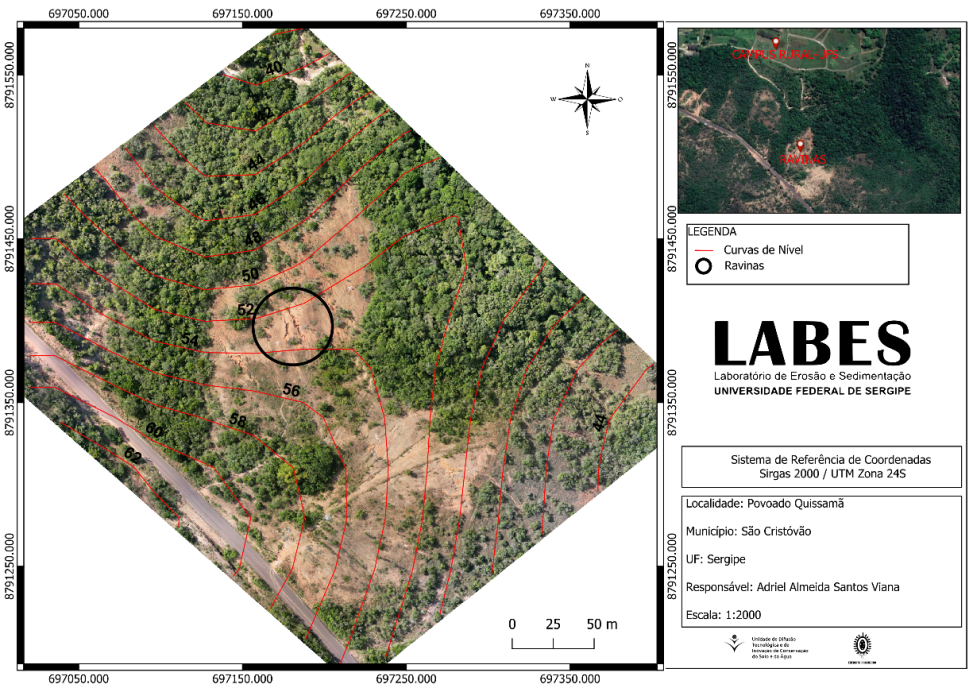
\includegraphics[width=0.85\textwidth]{figuras/fig_00a_area_estudo_aerea.png}\\[6pt]
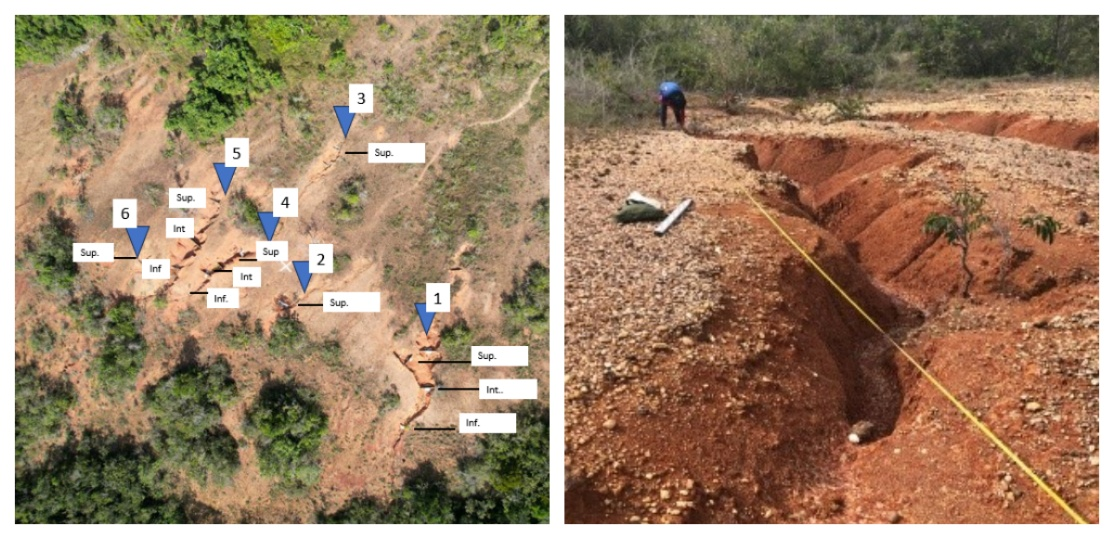
\includegraphics[width=0.85\textwidth]{figuras/fig_00b_feicoes_drone_campo.jpeg}
\caption{Sítio experimental nos Tabuleiros Costeiros de Sergipe, nordeste do Brasil. (a)~Vista aérea mostrando a paisagem de pastagem degradada e a ocorrência de feições lineares de erosão no Plintossolo Háplico (linhas no mapa delimitam a área de estudo e não representam necessariamente fronteiras nacionais oficiais). (b)~Ortomosaico obtido por aeronave remotamente pilotada mostrando a distribuição espacial das feições erosivas mapeadas. (c)~Medição de campo dos parâmetros morfométricos (profundidade, largura e comprimento) em uma das feições ativas.}
\label{fig:area}
\end{figure}

Todas as propriedades de entrada do Plintossolo foram obtidas em medições de campo e análises laboratoriais conduzidas em amostras coletadas no sítio experimental. A velocidade de infiltração básica (VIB) foi determinada in situ por ensaios de infiltrômetro de duplo anel em três horizontes representativos (Ap, BAc e Bf), produzindo valores de 3,13, 1,53 e 1,59~cm/h, respectivamente, que confirmam que os horizontes plínticos e subplínticos impõem impedimento hidráulico bem abaixo do limiar de referência adotado ($\mathrm{VIB_{ref}} = 6{,}0$~cm/h). 

A saturação por alumínio ($m_{\mathrm{Al}}$) foi quantificada por análise rotineira de fertilidade do solo em amostras de cada horizonte genético, com valores de 15,2\% no Ap a 99,2\% no Bf, gradiente vertical consistente com a lixiviação progressiva de bases e a concentração de alumínio trocável em profundidade. 

Os parâmetros geotécnicos (coesão efetiva $c = 13{,}02$~kPa, ângulo de atrito interno $\phi = 34{,}93^\circ$ e peso específico saturado $\gamma_{\mathrm{sat}} = 19{,}93$~kN/m$^3$) foram determinados por ensaio de cisalhamento direto (ASTM D3080) em amostras indeformadas extraídas do horizonte Bt sob condições saturadas. 

A erodibilidade $K_{\mathrm{RUSLE}} = 0{,}035$~t\,h\,MJ$^{-1}$\,mm$^{-1}$ foi estimada a partir da granulometria, do teor de matéria orgânica, do código de estrutura e da classe de permeabilidade do horizonte superficial usando o nomograma padrão \citep{wischmeier_et_al_1971}. Esses valores derivados de campo constituem o conjunto primário de entrada para os cinco testes computacionais (Tabela~\ref{tab:profiles}, coluna ``Plintossolo (campo)'').

Dois perfis virtuais (Latossolo e Argissolo) foram parametrizados a partir de valores medianos da literatura regional para VIB, saturação por alumínio, propriedades geotécnicas e $K_{\mathrm{RUSLE}}$ \citep{silva_et_al_2009,bertoni_lombardi_neto_2017}. O Latossolo opera como controle negativo ($\alpha \approx \beta \approx \gamma \approx 1$), representando solos bem drenados sem impedimento hidráulico, toxicidade ou feições erosivas profundas, ao passo que o Argissolo funciona como controle parcial, compartilhando impedimento hidráulico moderado no horizonte Bt mas sem plintita ou toxicidade alumínica extrema. Nenhuma medição de campo foi conduzida nessas duas classes; seu papel é exclusivamente computacional, servindo como referências frente às quais a amplificação do Plintossolo é avaliada.

\begin{table}[htbp]
\centering
\caption{Propriedades dos três perfis de solo utilizados nas simulações. Os valores do Plintossolo foram obtidos em medições de campo.}
\label{tab:profiles}
\small
\begin{tabular}{@{}l r r r@{}}
\toprule
Propriedade & Plintossolo (campo) & Latossolo (virtual) & Argissolo (virtual) \\
\midrule
VIB superior (cm/h) & 3,13 & 12,0 & 4,5 \\
VIB intermediária (cm/h) & 1,53 & 9,0 & 2,5 \\
VIB inferior (cm/h) & 1,59 & 7,0 & 2,8 \\
$K_{\mathrm{sat,ef}}$ (cm/h) & 0,50 & 8,0 & 1,0 \\
$m_{\mathrm{Al}}$ Ap (\%) & 15,2 & 10,0 & 20,0 \\
$m_{\mathrm{Al}}$ subsuperficial (\%) & 84--99 & 20,0 & 45,0 \\
$c$ (kPa, saturada) & 13,02 & 30,0 & 18,0 \\
$\phi$ ($^\circ$) & 34,93 & 30,0 & 32,0 \\
$\gamma_{\mathrm{sat}}$ (kN/m$^3$) & 19,93 & 18,0 & 19,0 \\
$H_c$ (m) & 3,35 & 5,77$^a$ & 4,33$^a$ \\
$H/H_c$ médio & 0,28 & 0,00 & 0,08 \\
$K_{\mathrm{RUSLE}}$ (t\,h\,MJ$^{-1}$\,mm$^{-1}$) & 0,035 & 0,015 & 0,025 \\
\bottomrule
\end{tabular}

\noindent $^a$ Calculado pela Eq.~\ref{eq:hc}.
\end{table}

\subsection{Campanha exploratória em talude com paliçadas baixas de pedra}
\label{sec:field-palisades}

A campanha exploratória foi instalada em um talude de Plintossolo adjacente ao sítio-alvo, sob pastagem degradada e declividade de 22$^{\circ}$. A montagem usou nove rampas reduzidas de 2,40~m $\times$ 0,50~m, cada uma com área de 1,20~m$^2$, das quais sete permaneceram sob solo descoberto e duas receberam paliçadas baixas de pedra, com aproximadamente 20~cm de fragmentos granulares dispostos transversalmente ao fluxo. 

Os tubos coletores foram posicionados na base das rampas para reter sedimento mobilizado por chuva natural, enquanto o bloco indeformado extraído do talude forneceu os parâmetros de cisalhamento direto usados na estimativa de $H_c$ (Fig.~\ref{fig:sitio}). Essa montagem foi destinada a estimar o envelope de ruído observacional e um \emph{prior} de cobertura-manejo para calibrações posteriores de $K_{\mathrm{plint}} \cdot C \cdot P$.

\begin{figure}[htbp]
\centering
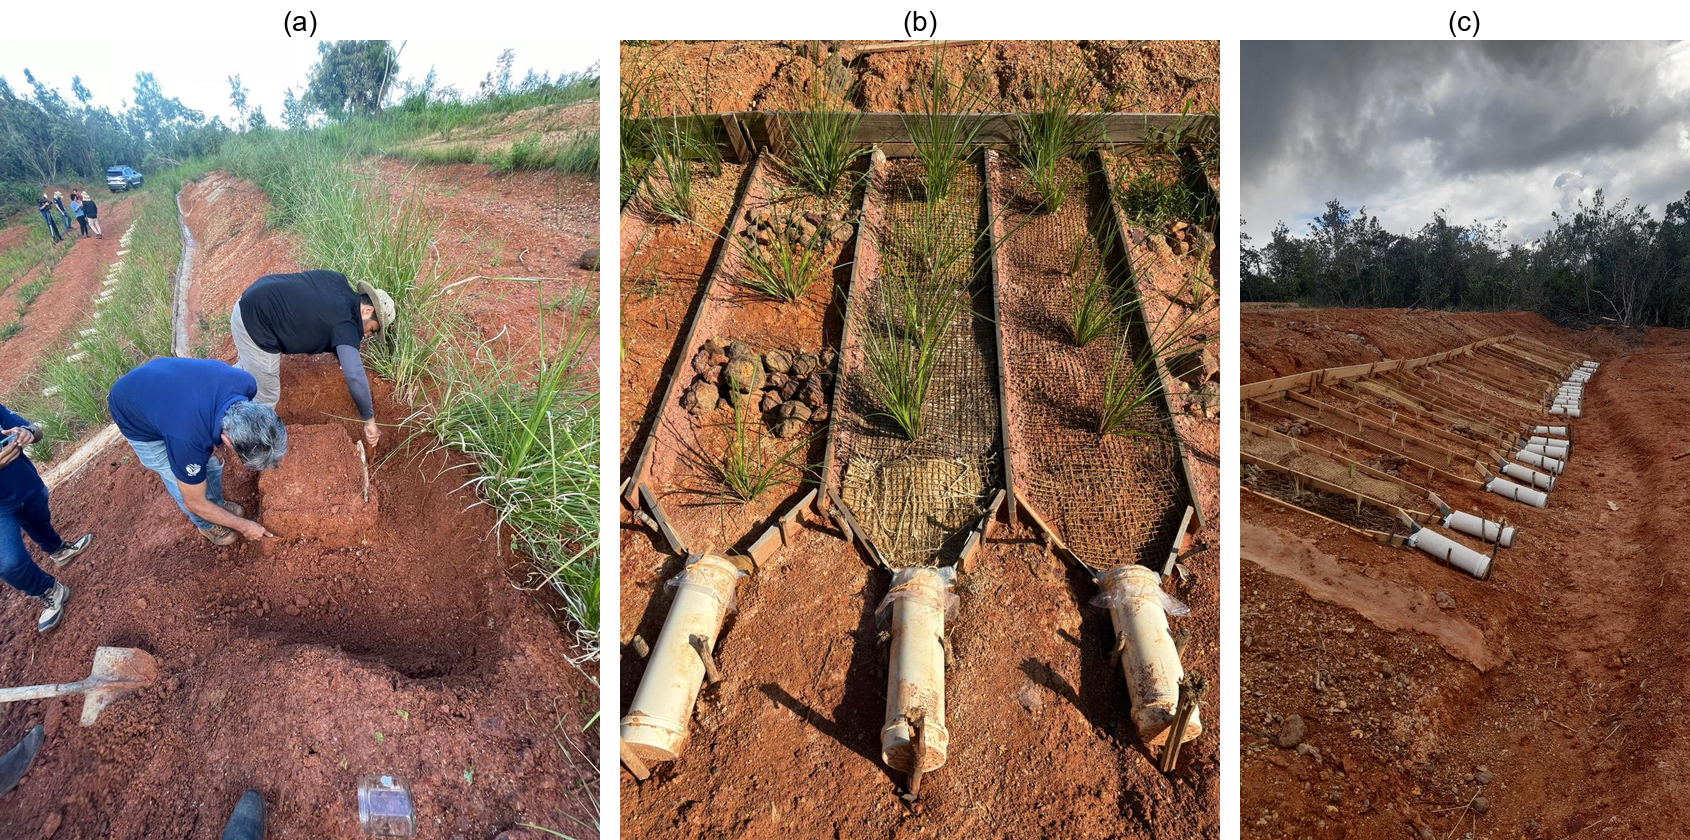
\includegraphics[width=\textwidth]{figuras/fig_09_sitio_experimental.png}
\caption{Montagem exploratória em talude de Plintossolo usada para comparar solo descoberto e paliçadas baixas de pedra. (a)~Bloco indeformado extraído para ensaio de cisalhamento direto, (b)~Tubos coletores de sedimento posicionados na base das rampas reduzidas e (c)~Talude com parcelas de solo descoberto e paliçadas baixas de pedra.}
\label{fig:sitio}
\end{figure}

\subsection{Parâmetros-alvo da calibração sintética}

Para os testes que requerem valores ``verdadeiros'' conhecidos, adotaram-se: $n_1 = 1{,}0$, $\beta_{\max} = 2{,}5$, $k_2 = 0{,}10$, $k_3 = 3{,}0$, $n_3 = 2{,}0$. Esses valores foram escolhidos dentro de faixas fisicamente plausíveis, sem a pretensão de representar os parâmetros reais do sítio (que só serão conhecidos após a calibração de campo).

\subsection{Teste~1: Calibração para recuperação de parâmetros}

O objetivo é verificar se o protocolo de calibração sequencial em quatro passos proposto recupera os cinco parâmetros conhecidos a partir de dados ruidosos. $\delta_{\mathrm{obs}}$ sintético foi gerado para 42 parcelas virtuais (16 Plintossolo, 12 Latossolo, 14 Argissolo) multiplicando $\delta_{\mathrm{verdadeiro}}$ por ruído gaussiano multiplicativo com CV de 10--30\%, de modo que $\delta_{\mathrm{obs}} = \delta_{\mathrm{verdadeiro}} \times (1 + \varepsilon)$ com $\varepsilon \sim N(0, \mathrm{CV}^2)$, truncado em $\delta_{\mathrm{obs}} > 0$ por admissibilidade física (nenhuma realização violou essa restrição nas 30 réplicas).

O protocolo de calibração segue a sequência de campo: verificação do controle negativo ($\delta_{\mathrm{Lat}} \approx 1$), estimação marginal de $\alpha$ via Argissolo, calibração de $\beta$ via contraste de horizontes do Plintossolo e calibração de $\gamma$ via resíduo geotécnico, seguidas por otimização simultânea via Levenberg--Marquardt. Cada nível de CV foi replicado 30 vezes.

\subsection{Teste~2: Análise global de sensibilidade (Sobol)}

Índices de Sobol de primeira ordem ($S_1$) e total ($S_T$) \citep{sobol_2001} foram calculados para quantificar a contribuição de cada parâmetro à variância de $\delta$ em quatro cenários representativos: Plintossolo intermediário (VIB = 1,53, $m = 84\%$, $H/H_c = 0{,}33$), Plintossolo superior (VIB = 3,13, $m = 15\%$, $H/H_c = 0{,}12$), Argissolo (VIB = 2,5, $m = 45\%$, $H/H_c = 0{,}08$) e Latossolo (VIB = 9,0, $m = 20\%$, $H/H_c = 0$). 

A amostragem de Saltelli \citep{saltelli_et_al_2004} com $N = 1024$ gerou 12\,288 avaliações do modelo. Os cinco parâmetros foram amostrados como variáveis uniformes independentes, premissa sustentada pela formulação multiplicativa em que $\alpha$, $\beta$ e $\gamma$ representam mecanismos fisicamente distintos sem correlação paramétrica a priori. Os limites de busca foram $n_1 \in [0{,}1; 3{,}0]$, $\beta_{\max} \in [1{,}1; 5{,}0]$, $k_2 \in [0{,}01; 0{,}50]$, $k_3 \in [0{,}5; 10{,}0]$ e $n_3 \in [1{,}0; 4{,}0]$.

\subsection{Teste~3: Estabilidade de talude e validação de $\gamma$}
\label{sec:test3}

O fator de segurança de Rankine (FS) \citep{rankine_1857} para cortes verticais foi calculado para $H/H_c$ de 0,05 a 0,95 sob seis níveis de pressão neutra relativa ($r_u = 0$ a 0,5), usando os parâmetros geotécnicos de campo do Plintossolo. O volume mobilizado por uma cunha de ruptura plana foi normalizado e modelado como proxy de contribuição geotécnica ($\delta_{\mathrm{geo}} \propto V_{\mathrm{norm}}/\mathrm{FS}$). A função $\gamma = 1 + k_3(H/H_c)^{n_3}$ foi ajustada ao proxy por mínimos quadrados não lineares, e o FS correspondente a cada uma das seis feições reais (F1--F6) foi verificado.

\subsection{Teste~4: Geração de infiltração e escoamento (Green--Ampt)}

O modelo de infiltração de Green--Ampt \citep{green_ampt_1911} foi aplicado aos três perfis de solo sob eventos de chuva com $I_{30}$ de 5--100~mm/h e duração de 60~min. O $K_{\mathrm{sat}}$ efetivo de cada perfil corresponde ao horizonte limitante (mínimo entre camadas). O coeficiente de escoamento (CE) foi calculado e a razão $\mathrm{CE}_{\mathrm{solo}}/\mathrm{CE}_{\mathrm{Latossolo}}$ comparada com $\alpha(\mathrm{VIB})$ para diferentes valores de $n_1$, avaliando a consistência entre o modelo hidráulico analítico e a forma funcional proposta.

\subsection{Teste~5: Erosão virtual (modelo simplificado tipo WEPP)}

O escoamento gerado pelo modelo de Green--Ampt foi convertido em tensão cisalhante de fundo ($\tau = \rho g h S$, fluxo uniforme (equação de Manning)) e em perda de solo via modelo de desprendimento ($D = k_r(\tau - \tau_c)$ para $\tau > \tau_c$). A erodibilidade $K_{\mathrm{obs}}$ foi invertida pela relação USLE ($K_{\mathrm{obs}} = A/(EI_{30} \times LS)$) e a discrepância $\delta_{\mathrm{obs}} = K_{\mathrm{obs}}/K_{\mathrm{RUSLE}}$ comparada com $\delta_{\mathrm{mod}}$ predito pela Eq.~\ref{eq:kplint} usando os parâmetros-alvo da Seção~3.2. Os parâmetros intrínsecos de erodibilidade ($k_r$, $\tau_c$) foram estimados da literatura para solos tropicais.

%% ================================================================
%%  4. RESULTADOS E DISCUSSÃO
%% ================================================================
\section{Resultados e discussão}
\label{sec:results}

\subsection{Resposta dos fatores no Plintossolo de campo}

O Plintossolo de Sergipe (Tabela~\ref{tab:profiles}) e as seis feições erosivas mapeadas em campo (Fig.~\ref{fig:area}b--c) fornecem os três atributos pedológicos diretamente mensuráveis que parametrizam $K_{\mathrm{plint}}$, dispensando etapa intermediária de modelagem hidrológica detalhada.

A VIB do horizonte BAc, de 1,53~cm/h, gera $\alpha = (6{,}0/1{,}53)^{n_1} = 3{,}92^{n_1}$. Para $n_1 = 1$, o impedimento subsuperficial amplifica a erodibilidade efetiva em quase quatro vezes em relação a um solo na VIB de referência, magnitude da mesma ordem do erro sistemático que o nomograma original comete em solos tropicais com horizonte limitante \citep{alewell_et_al_2019}. Em um Latossolo Vermelho-Amarelo típico, com VIB de 9~cm/h, $\alpha = 1$ porque $\mathrm{VIB} > \mathrm{VIB_{ref}}$, e a mesma equação opera como controle negativo em solos bem drenados sem reparametrização adicional. A consistência hidrológica desse contraste é retomada no Teste~4.

O fator fitotóxico apresenta gradiente vertical pronunciado. O horizonte Ap, com $m_{\mathrm{Al}} = 15{,}2\%$, gera $\beta \approx 1{,}04$ para $\beta_{\max} = 2{,}5$ e $k_2 = 0{,}10$, praticamente sem amplificação. O horizonte BAc, em contraste, alcança $m_{\mathrm{Al}} = 99{,}2\%$ e $\beta \approx 2{,}47$, próximo do máximo. A superfície ainda pode sustentar cobertura esparsa, ao passo que os horizontes expostos nos taludes ficam essencialmente desprovidos de proteção radicular contra o desprendimento por fluxo concentrado \citep{vannoppen_2015}, condição que a RUSLE clássica aproxima apenas indiretamente pelo fator $C$.

Os parâmetros geotécnicos medidos ($c = 13{,}02$~kPa, $\phi = 34{,}93^\circ$, $\gamma_{\mathrm{sat}} = 19{,}93$~kN/m$^3$) resultam em $H_c = 3{,}35$~m. As seis feições têm profundidades de 0,40--1,50~m, correspondentes a $H/H_c = 0{,}12$--0,45, intervalo no qual $\gamma$ permanece próximo de~1 e o colapso geotécnico ainda não é o mecanismo dominante de perda de solo. Em ravinas regionais com profundidade superior a 2~m ($H/H_c > 0{,}6$), $\gamma$ pode contribuir substancialmente para a amplificação total, justificando a inclusão desse termo na RUSLE estendida. A verificação do fator de segurança por feature e o ajuste de $\gamma$ são tratados no Teste~3.

\subsection{Recuperação de parâmetros (Teste~1)}

Os três parâmetros hidráulico-biológicos ($n_1$, $\beta_{\max}$, $k_2$) foram recuperados pelo protocolo sequencial com viés relativo mediano inferior a 15\% para todos os níveis de ruído sintético testados (Fig.~\ref{fig:calibracao}), condição necessária para que $K_{\mathrm{plint}}$ opere como fator estendido da RUSLE em dados de campo com ruído realista. A precisão decresceu na ordem $n_1 > k_2 > \beta_{\max}$ sob CV de 30\%, e a maior acurácia de $n_1$ (mediana 1,01--1,18 versus 1,0) é coerente com o domínio do termo hidráulico na variância de $\delta$ no Plintossolo, com implicação direta sobre a perda de solo predita pela RUSLE corrigida porque erros residuais nesse expoente se propagam multiplicativamente para a estimativa final.

A amplificação máxima de toxicidade ($\beta_{\max} = 2{,}28$--2,85, verdadeiro 2,5) e a taxa de transição ($k_2 = 0{,}11$--0,13, verdadeiro 0,10) exibiram vieses comparáveis. A faixa estreita de $m_{\mathrm{Al}}$ nos horizontes expostos atenua a propagação desses vieses para $K_{\mathrm{plint}}$, embora a dispersão de $\beta_{\max}$ tenha aumentado com o nível de ruído sem gerar tendência sistemática.

\begin{figure}[htbp]
\centering

\includegraphics[width=0.9\textwidth]{figuras/fig_01_calibracao_sintetica.png}
\caption{Viés relativo mediano dos parâmetros estimados em função do coeficiente de variação (CV) do ruído sintético.}
\label{fig:calibracao}
\end{figure}

Os parâmetros $k_3$ e $n_3$ exibiram alta dispersão e tendência a convergir para os limites superiores das faixas de busca (Fig.~\ref{fig:boxplot}), com medianas de 14,9 e 3,9 respectivamente para CV = 30\% (verdadeiros 3,0 e 2,0). Para $H/H_c = 0{,}12$--0,45, o produto $k_3 \times (H/H_c)^{n_3}$ admite múltiplas combinações com $\gamma$ próximo de 1,0, gerando equifinalidade. O fenômeno é análogo ao descrito por \citet{beven_freer_2001} para modelos hidrológicos mecanísticos e foi formalizado por \citet{beven_2006} como propriedade intrínseca de modelos sobreparametrizados.

Para o usuário operacional da RUSLE, essa equifinalidade significa que o termo $\gamma$ não pode ser calibrado apenas com feições rasas e que estimativas em ravinas profundas devem usar priors geotécnicos. \citet{her_chaubey_2015} demonstraram que a equifinalidade tende a diminuir quando os dados cobrem a faixa dinâmica do modelo, sugerindo que feições com $H/H_c > 0{,}45$ precisam ser monitoradas para reduzir a indeterminação de $k_3$ e $n_3$. Um arcabouço bayesiano com priors derivados da análise de Rankine (Material Suplementar~S1) pode restringir a distribuição posterior e mitigar a equifinalidade aqui identificada.

Como os dados de campo do Plintossolo não contêm feições com $H/H_c > 0{,}45$, a calibração desse fator requer monitoramento de feições com profundidade superior a 1,5~m ou modelagem geotécnica complementar. Essa restrição não inviabiliza o uso da estrutura $K_{\mathrm{plint}}$ na RUSLE, mas delimita a faixa de profundidade em que o termo $\gamma$ pode ser tomado como ajustado.

\begin{figure}[htbp]
\centering

\includegraphics[width=\textwidth]{figuras/fig_02_boxplot_parametros.png}
\caption{Distribuição dos parâmetros estimados em 30 réplicas por nível de ruído. Linhas vermelhas tracejadas indicam os valores verdadeiros.}
\label{fig:boxplot}
\end{figure}

O controle negativo (Latossolo) produziu $\delta_{\mathrm{Lat}}$ mediano de 1,04--1,07 em todos os níveis de CV, confirmando que o modelo prevê corretamente $\delta \approx 1$ quando as três condições amplificadoras estão ausentes. O comportamento decorre da formulação multiplicativa, em que $\alpha = 1$ para $\mathrm{VIB} \geq \mathrm{VIB_{ref}}$, $\beta \approx 1$ para $m_{\mathrm{Al}} < 50\%$ e $\gamma = 1$ para $H/H_c = 0$, de modo que o ruído residual em $\delta$ é atribuível apenas à propagação numérica.

A proximidade à unidade reforça a especificidade pedológica do fator e é coerente com o achado de que Latossolos profundos tendem a apresentar erodibilidade próxima ou inferior à estimativa do nomograma, em razão da macroagregação por óxidos de ferro e alumínio \citep{cassol_et_al_2023}. A assimetria do erro do nomograma entre classes pedológicas reforça que $K_{\mathrm{plint}}$ atua nas duas direções da RUSLE clássica: \citet{auerswald_et_al_2014} demonstraram superestimação em solos com agregados estáveis e alta condutividade, condição típica de Latossolos, ao passo que \citet{ostovari_et_al_2016} observaram subestimação em solos calcários com impedimento subsuperficial, padrão análogo ao dos Plintossolos. O desenho experimental com controle negativo é, portanto, indispensável para isolar os efeitos de cada amplificador durante a calibração de campo.

\subsection{Hierarquia de sensibilidade (Teste~2)}

O expoente hidráulico $n_1$ concentrou 63\% da variância de $\delta$ no cenário Plintossolo intermediário ($\mathrm{VIB} = 1{,}53$~cm/h, $m = 84\%$, $H/H_c = 0{,}33$), com $S_T = 0{,}84$ indicando interações relevantes com $\beta_{\max}$ e $n_3$ (Fig.~\ref{fig:sobol}). Essa hierarquia orienta onde alocar esforço de medição na atualização da RUSLE para Plintossolos, dado que parâmetros de baixa sensibilidade podem ser fixados por evidência independente sem perda preditiva \citep{saltelli_et_al_2004}, em padrão consistente com a análise de \citet{chaves_nearing_1991} no WEPP, onde erodibilidade em entressulcos e condutividade hidráulica respondem por mais de 70\% da variância da perda de solo predita. No cenário Plintossolo superior ($\mathrm{VIB} = 3{,}13$~cm/h), $n_1$ domina ainda mais marcadamente ($S_1 = 0{,}78$, $S_T = 0{,}85$) porque o gradiente menor reduz a sensibilidade relativa dos demais termos.

\begin{figure}[htbp]
\centering

\includegraphics[width=\textwidth]{figuras/fig_03_sensibilidade_sobol.png}
\caption{Índices de sensibilidade de Sobol de primeira ordem ($S_1$) e total ($S_T$) para quatro cenários pedológicos.}
\label{fig:sobol}
\end{figure}

O Argissolo apresentou padrão semelhante ($S_1$ de $n_1 = 0{,}79$), indicando que em solos com $\mathrm{VIB} < \mathrm{VIB_{ref}}$ o regime hidráulico é o mecanismo dominante de amplificação. O Latossolo, operando com $\mathrm{VIB} > \mathrm{VIB_{ref}}$ (portanto $\alpha = 1$), transfere a variância para $k_2$ ($S_1 = 0{,}70$, $S_T = 0{,}93$). A concordância entre hierarquia paramétrica e mecanismo pedológico esperado indica consistência interna do modelo e que o desenho multiclasse é necessário para uma calibração equilibrada.

O domínio do mecanismo hidráulico converge com \citet{francois_et_al_2024}, que identificaram $K$ como o parâmetro mais sensível da RUSLE no sul da Bahia, e com \citet{alewell_et_al_2019}, para quem a transferibilidade do nomograma a ambientes tropicais é limitada pela ausência de representação de processos subsuperficiais. Em parcelas no sul da Itália, \citet{bagarello_et_al_2012} mediram erodibilidade que excedeu sistematicamente as estimativas do nomograma em solos com horizonte argiloso subsuperficial. A semelhança do diagnóstico em províncias geomorfológicas distintas reforça que o impedimento hidráulico é amplificador reconhecido de $K$ em escala global, ainda que a cimentação por óxidos de ferro constitua mecanismo adicional próprio dos Plintossolos.

A matriz de interações de segunda ordem ($S_2$) para o Plintossolo intermediário (Fig.~\ref{fig:interacoes}) indicou interação relevante entre $n_1$ e $\beta_{\max}$ ($S_2 \approx 0{,}05$--0,10) e entre $k_3$ e $n_3$ ($S_2 \approx 0{,}02$), corroborando a equifinalidade identificada na calibração sintética. A interação $n_1$--$\beta_{\max}$ tem interpretação física direta, já que perfis com baixa VIB e alto $m_{\mathrm{Al}}$ ativam ambos os termos amplificadores simultaneamente. A interação $k_3$--$n_3$, por sua vez, é puramente paramétrica e decorre da superfície de resposta achatada de $\gamma$ no intervalo $H/H_c < 0{,}45$.

A distinção entre interações mecanísticas e indeterminação espúria orienta o desenho de parcelas para calibrar a RUSLE corrigida. As interações reais exigem parcelas que capturem a covariância entre infiltração e toxicidade, enquanto as espúrias podem ser mitigadas por restrição prévia do espaço paramétrico via análise geotécnica.

\begin{figure}[htbp]
\centering
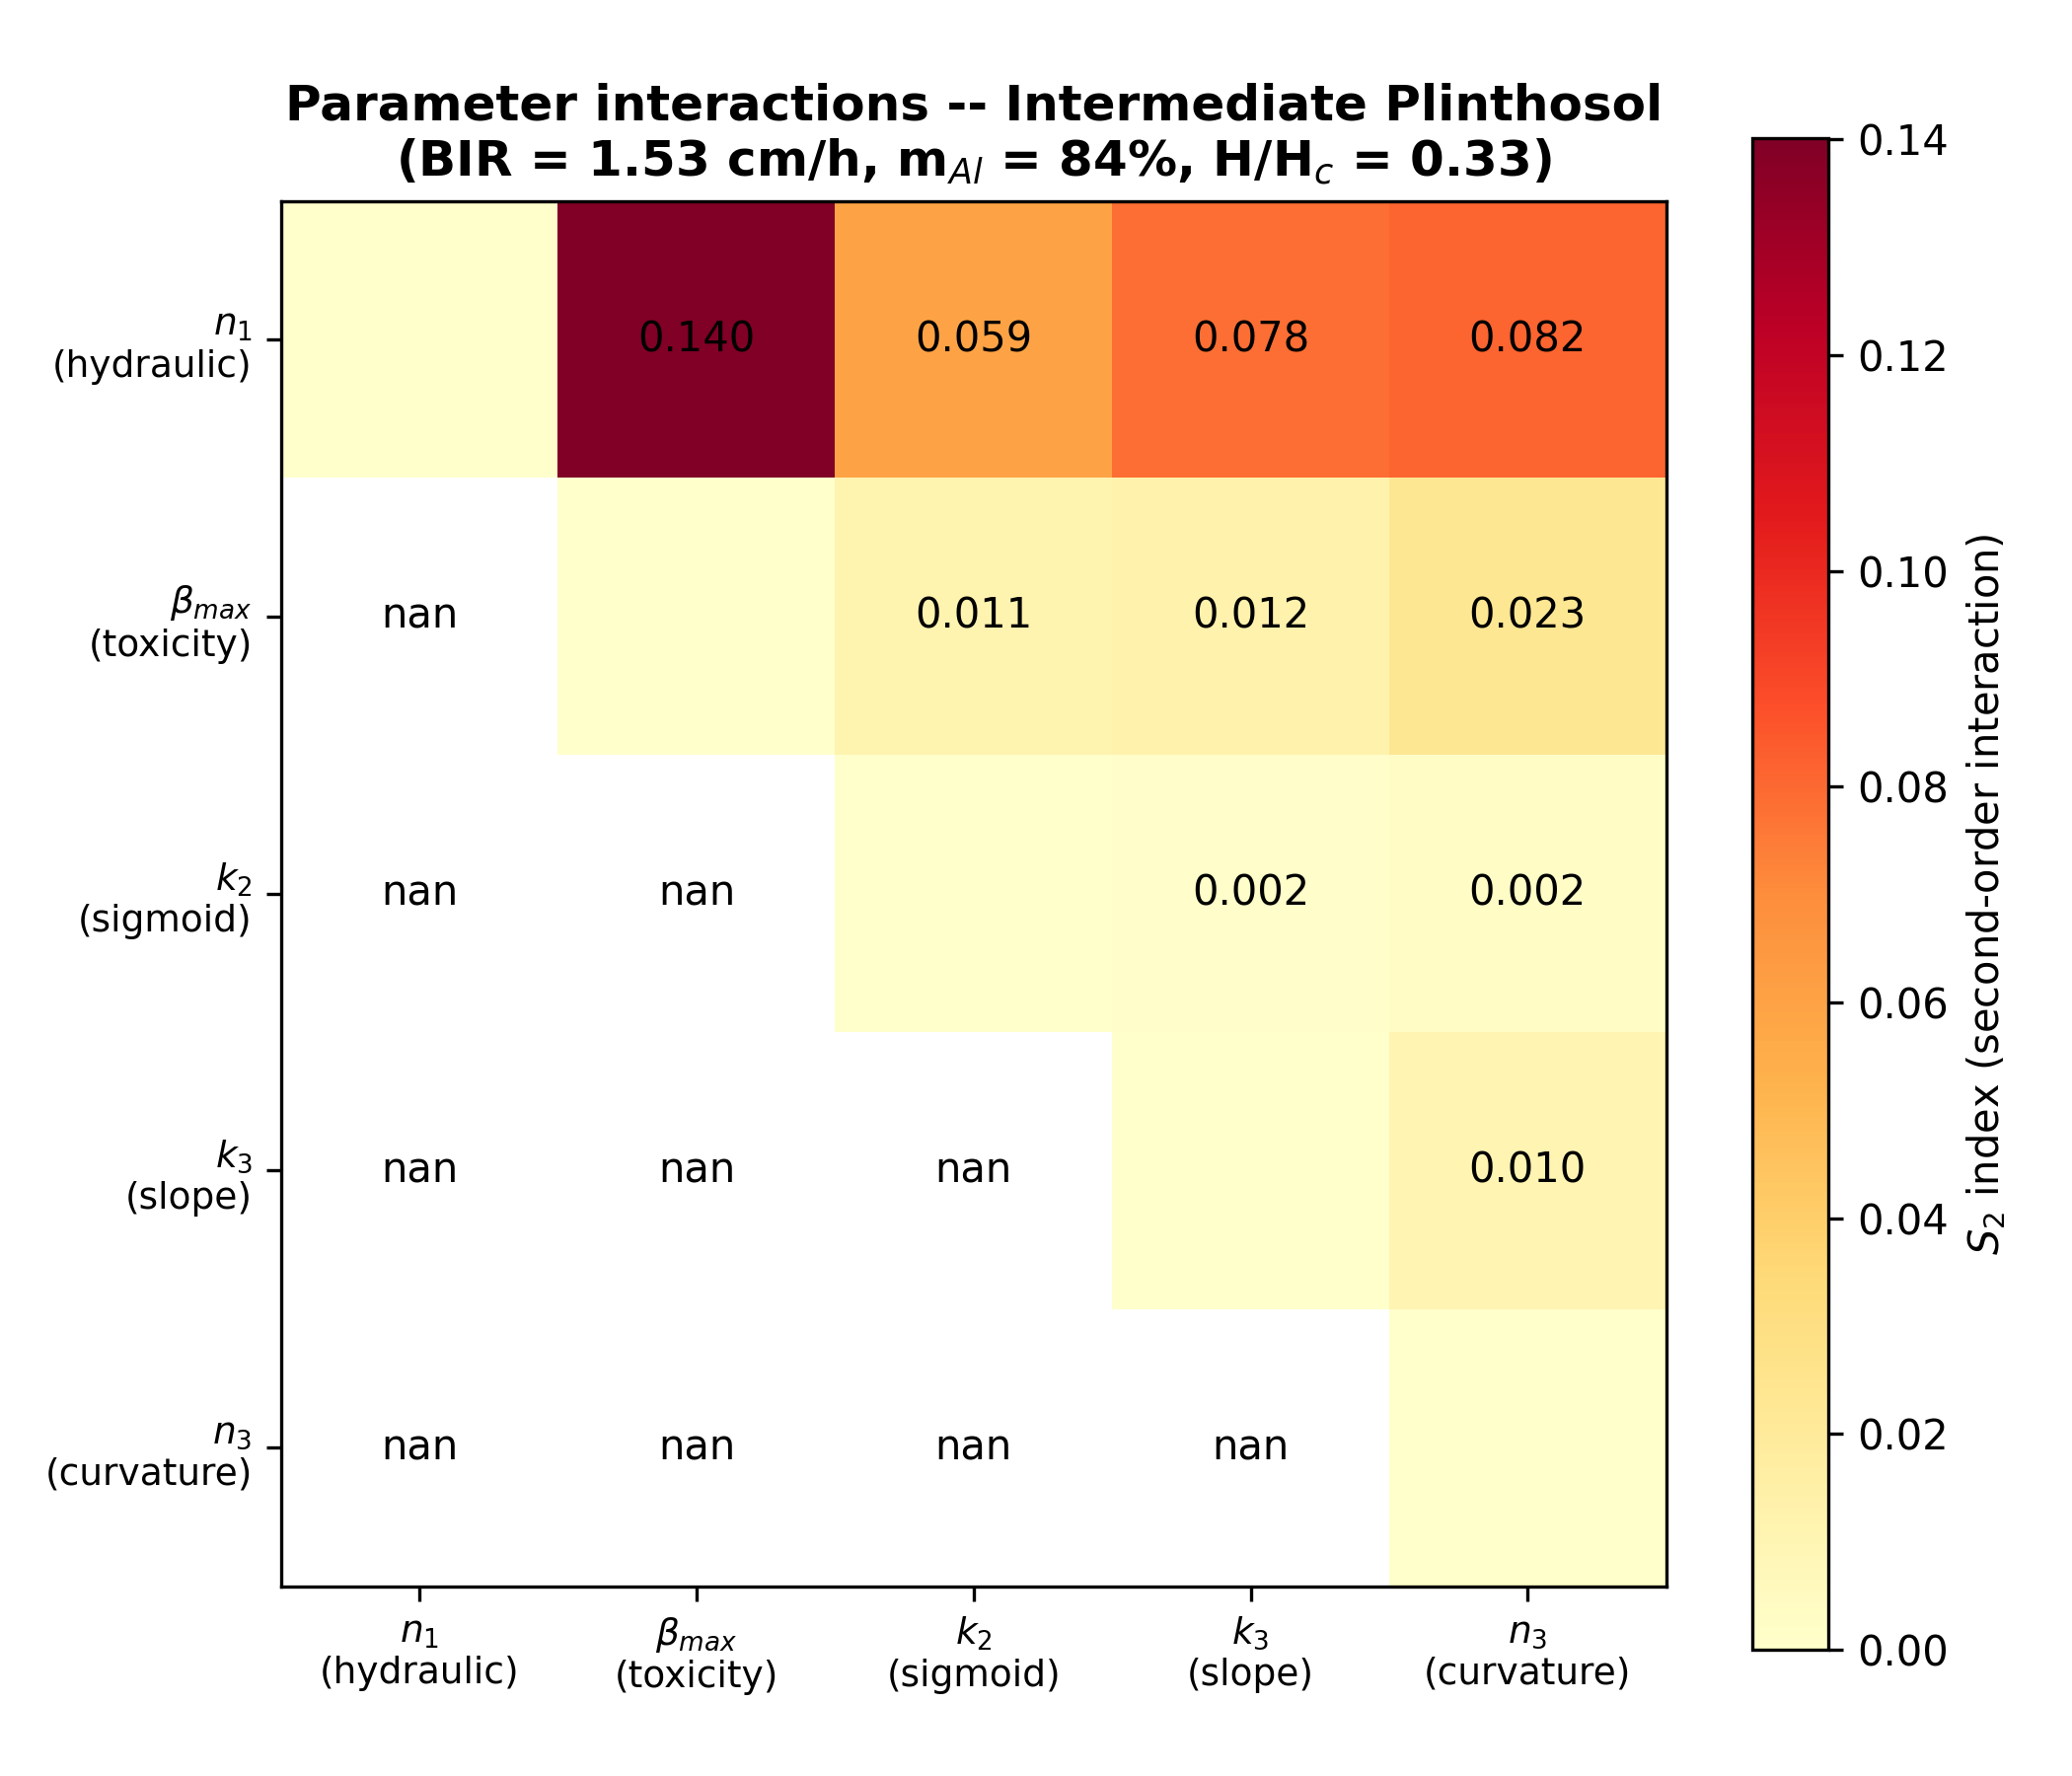
\includegraphics[width=0.7\textwidth]{figuras/fig_04_interacoes_s2.png}
\caption{Matriz de interações de segunda ordem ($S_2$) de Sobol para o cenário Plintossolo intermediário ($\mathrm{VIB} = 1{,}53$~cm/h, saturação por alumínio $= 84\%$, $H/H_c = 0{,}33$).}
\label{fig:interacoes}
\end{figure}

\subsection{Validação geotécnica de $\gamma$ (Teste~3)}

O ajuste de $\gamma = 1 + k_3(H/H_c)^{n_3}$ ao proxy $\delta_{\mathrm{geo}}$ derivado de Rankine convergiu para $k_3 = 6{,}50$ e $n_3 = 4{,}51$ (Fig.~\ref{fig:taludes}), parametrizando o termo geotécnico exigido pela RUSLE estendida em ravinas onde o colapso se soma ao desprendimento hidráulico, valores substancialmente superiores aos alvos da calibração sintética ($3{,}0$ e $2{,}0$). A divergência é fisicamente coerente porque a contribuição volumétrica do colapso cresce mais rapidamente com $H/H_c$ do que a expansão quadrática originalmente proposta, em razão da dependência cúbica ou quártica do volume da cunha em relação à altura da parede \citep{fredlund_rahardjo_1993}. O expoente $n_3 \approx 4{,}5$ implica que $\gamma$ permanece desprezível para $H/H_c < 0{,}3$ e cresce abruptamente acima desse limiar, consistente com a observação de campo de que apenas F4 ($H/H_c = 0{,}42$) e F5 (0,45) foram classificadas como ravinas incipientes pelo sistema fuzzy.

Em ravinas sobre sedimentos do Grupo Barreiras em Bananal (SP), \citet{oliveira_1991} identificou comportamento análogo, com transição entre erosão por fluxo concentrado e ruptura de massa acima de $H/H_c \approx 0{,}35$--0,40. No sudeste da Espanha, \citet{vandekerckhove_et_al_2003} quantificaram taxas de recuo de cabeçeira de 0,01--0,89~m/ano, com os valores mais altos em feições de paredes verticais e profundidade superior a 1,5~m, condição em que a instabilidade gravitacional supera o desprendimento hidráulico. Em modelo de recuo validado para razões $H/H_c$ elevadas, \citet{campo_bescos_et_al_2013} corroboraram essa relação ao identificarem componente de colapso superior à hidráulica, sustentando a não linearidade pronunciada ($n_3 > 4$) aqui observada.

\begin{figure}[htbp]
\centering
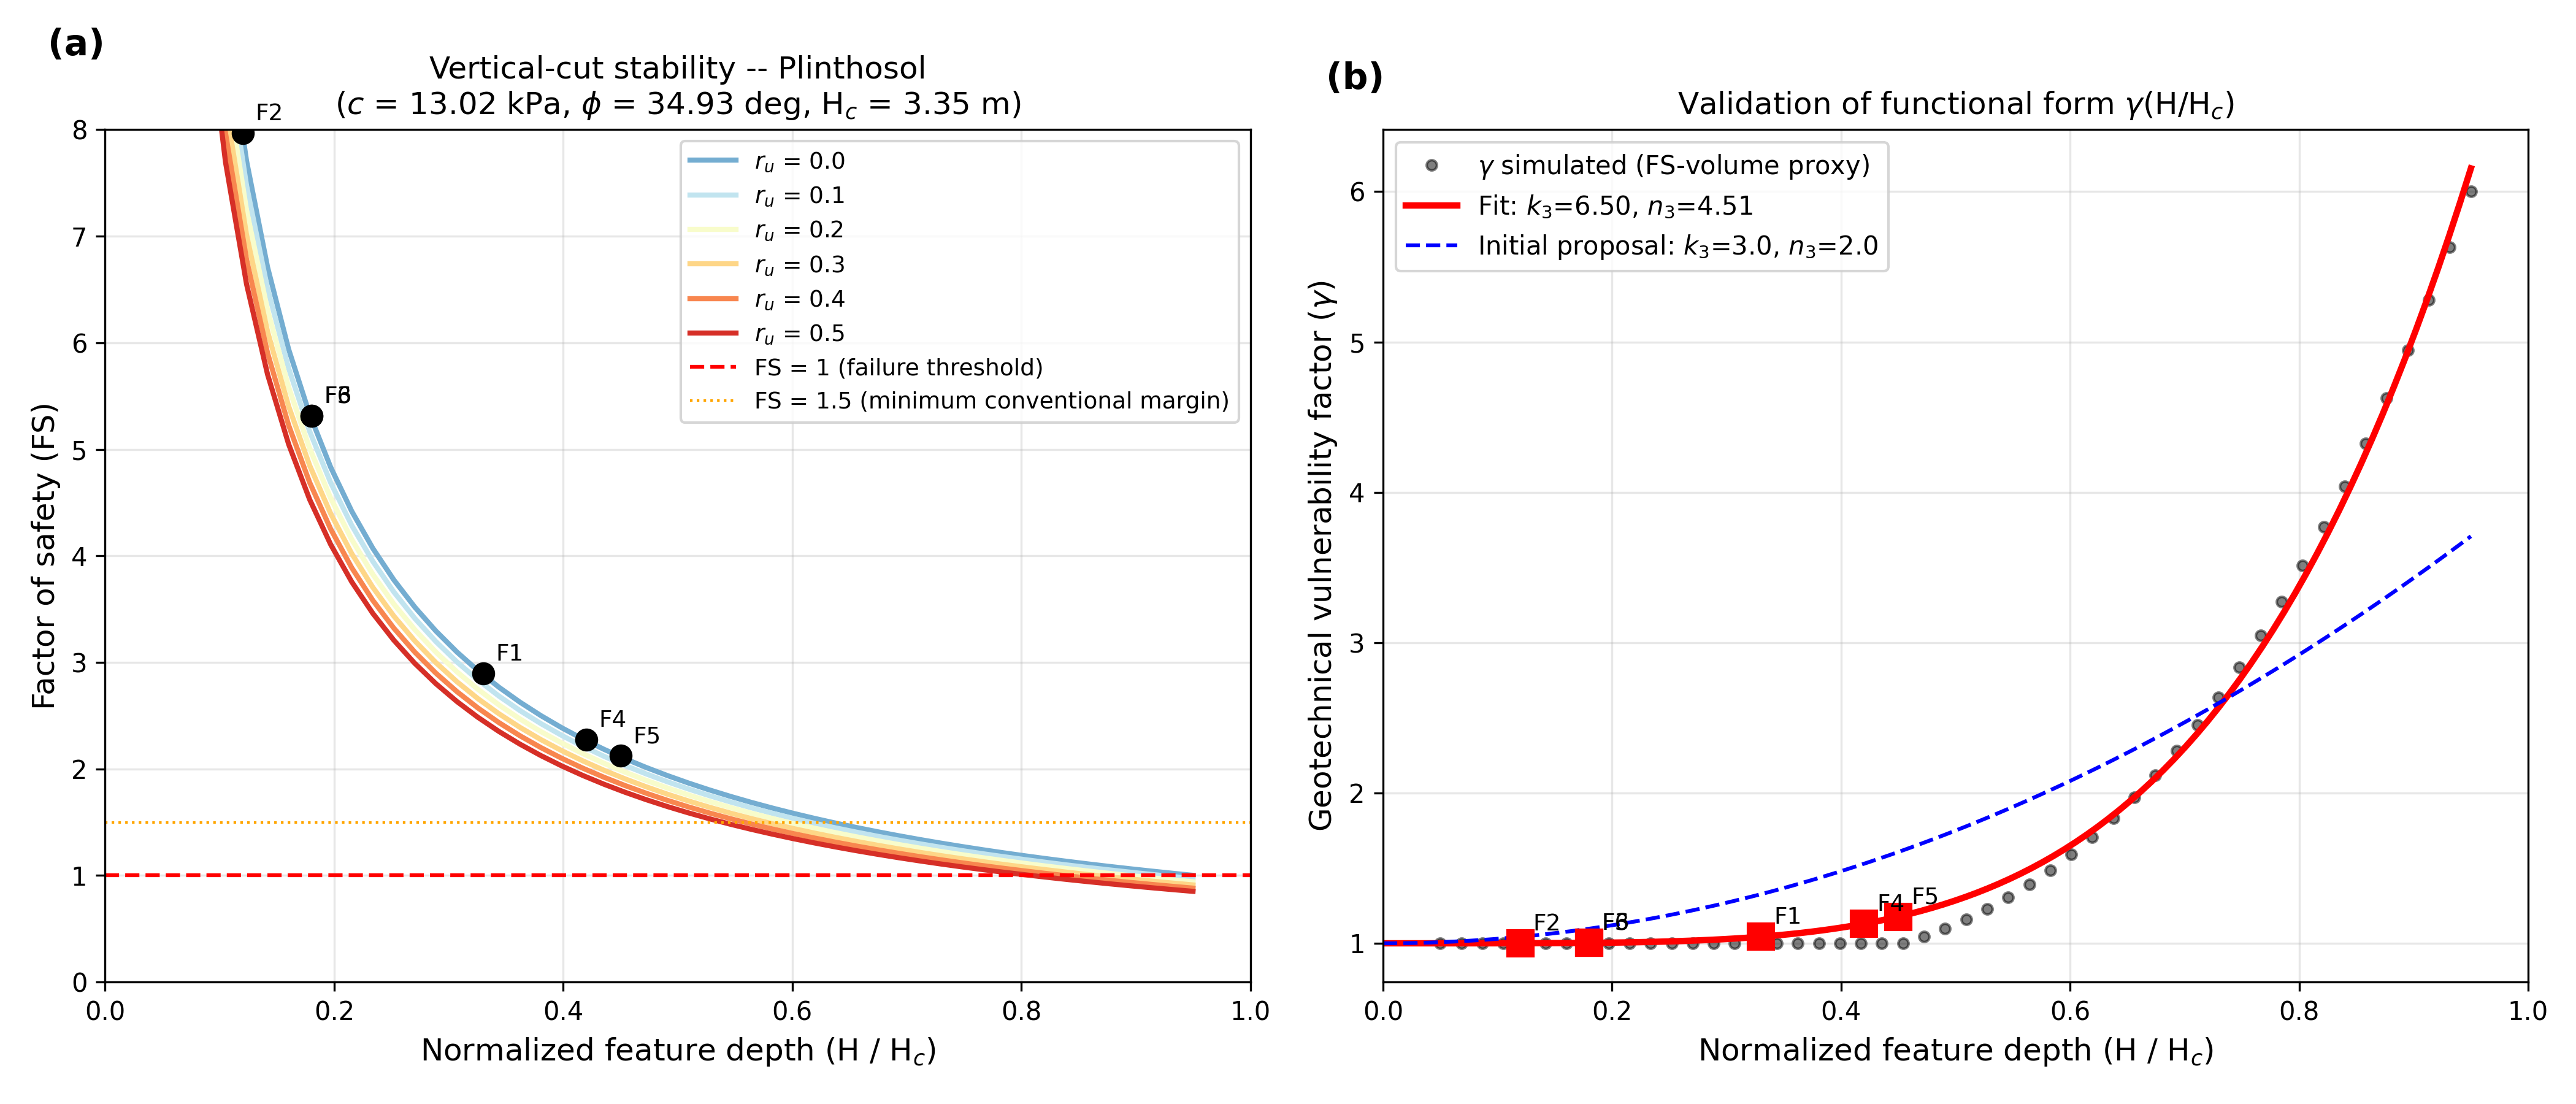
\includegraphics[width=\textwidth]{figuras/fig_05_estabilidade_taludes.png}
\caption{(a)~Fator de segurança de Rankine (FS) em função de $H/H_c$ sob diferentes pressões neutras relativas ($r_u$). (b)~Proxy $\delta_{\mathrm{geo}}$ e ajuste em potência $\gamma = 1 + 6{,}50 \times (H/H_c)^{4{,}51}$. Pontos vermelhos: feições reais F1--F6.}
\label{fig:taludes}
\end{figure}

O fator de segurança é sensível à pressão neutra relativa, decrescendo de 2,12 para 1,93 na F5 quando $r_u$ passa de 0 a 0,3. Sob saturação prolongada em eventos extremos, essa redução pode aproximar o FS da unidade e desencadear colapsos laterais que retroalimentam a perda de solo, mecanismo que \citet{vanmaercke_et_al_2021} identificaram como responsável por até 60\% do avanço volumétrico de ravinas em regiões subtropicais. A RUSLE corrigida pelo termo $\gamma$ acomoda esse processo sem exigir um modelo dinâmico de estabilidade.

Todas as seis feições reais apresentaram FS $>$\,2,0 para $r_u = 0$ e FS $>$\,1,8 para $r_u = 0{,}3$ (Tabela~\ref{tab:fs}), margem consistente com a classificação como ravinas sem colapso ativo segundo \citet{poesen_2018}. O $\gamma$ ajustado para a F5 ($H/H_c = 0{,}45$) atingiu 1,18, indicando 18\% de amplificação geotécnica sobre a erodibilidade basal, enquanto a F2 ($H/H_c = 0{,}12$) permanece em $\gamma = 1{,}00$. Para feições com $H/H_c > 0{,}6$, documentadas em ravinas regionais, $\gamma$ pode exceder 2,0, condição em que o mecanismo geotécnico contribuiria com magnitude comparável ou superior às amplificações hidráulica e fitotóxica e justificaria a inclusão obrigatória do termo na aplicação regional da RUSLE.

\begin{table}[htbp]
\centering
\caption{Fator de segurança e $\gamma$ ajustado para as seis feições erosivas reais.}
\label{tab:fs}
\small
\begin{tabular}{@{}c r r r r r@{}}
\toprule
Feição & $H$ (m) & $H/H_c$ & FS ($r_u = 0$) & FS ($r_u = 0{,}3$) & $\gamma$ ajustado \\
\midrule
F1 & 1,10 & 0,33 & 2,90 & 2,64 & 1,04 \\
F2 & 0,40 & 0,12 & 7,97 & 7,25 & 1,00 \\
F3 & 0,60 & 0,18 & 5,31 & 4,83 & 1,00 \\
F4 & 1,40 & 0,42 & 2,28 & 2,07 & 1,13 \\
F5 & 1,50 & 0,45 & 2,12 & 1,93 & 1,18 \\
F6 & 0,60 & 0,18 & 5,31 & 4,83 & 1,00 \\
\bottomrule
\end{tabular}
\end{table}

\subsection{Geração de escoamento e validação de $\alpha$ (Teste~4)}

O Plintossolo ($K_{\mathrm{sat,ef}} = 0{,}50$~cm/h, BAc limitante) gerou, sob o modelo de Green--Ampt, coeficiente de escoamento de 0,20 para $I_{30} = 30$~mm/h e 0,56 para $I_{30} = 60$~mm/h (Fig.~\ref{fig:infiltracao}a), refletindo o impedimento subsuperficial que converte a fração não infiltrada em escoamento hortoniano mesmo sob intensidades moderadas. A adoção do $K_{\mathrm{sat}}$ do horizonte limitante como condutividade efetiva segue \citet{wang_et_al_1999}, em que a camada menos permeável controla o tempo de empoçamento independentemente da condutividade da camada superior, premissa adequada a Plintossolos cujo horizonte plíntico tem condutividade uma a duas ordens de magnitude inferior à do horizonte A. O Argissolo ($K_{\mathrm{sat,ef}} = 1{,}0$~cm/h) produziu CE = 0,37 para $I_{30} = 60$~mm/h, intermediário entre os dois extremos e consistente com o impedimento parcial do horizonte Bt sem plintita.

\begin{figure}[htbp]
\centering

\includegraphics[width=\textwidth]{figuras/fig_06_infiltracao_escoamento.png}
\caption{(a)~Coeficiente de escoamento (CE) em função de $I_{30}$ para os três perfis (Green--Ampt, evento de 60~min). (b)~Razão CE/CE$_{\mathrm{Lat}}$ comparada com $\alpha$ teórico (Eq.~\ref{eq:alpha}) para três valores de $n_1$.}
\label{fig:infiltracao}
\end{figure}

O Latossolo ($K_{\mathrm{sat,ef}} = 8{,}0$~cm/h) não gerou escoamento em nenhuma das intensidades testadas (CE = 0 para $I_{30}$ até 100~mm/h), indicando que o limiar $\mathrm{VIB_{ref}} = 6$~cm/h é conservador e que solos com $K_{\mathrm{sat}}$ efetivo superior a esse nível tendem a operar integralmente em regime dominado por infiltração. O CE de 0,56 obtido para o Plintossolo é compatível com a magnitude esperada em solos cujo horizonte limitante apresenta $K_{\mathrm{sat}}$ inferior a 1~cm/h \citep{morgan_2005}, ao passo que a ausência de escoamento no Latossolo é coerente com solos profundos e bem drenados \citep{bertoni_lombardi_neto_2017}. A diferenciação sustenta o uso do Latossolo como controle negativo onde $K_{\mathrm{obs}} \approx K_{\mathrm{RUSLE}}$ e dispensa correção.

O hidrograma sob $I_{30} = 60$~mm/h (Fig.~\ref{fig:hidrograma}) ilustra a diferença temporal na geração de escoamento, com o Plintossolo atingindo regime estacionário em menos de 10~min e o Argissolo requerendo aproximadamente 25~min, reflexo da proporção inversa entre $K_{\mathrm{sat,ef}}$ e o tempo de empoçamento previsto pela teoria de excesso de infiltração \citep{horton_1933}. A ausência de escoamento no Latossolo durante todo o evento de 60~min é coerente com solos cujo $K_{\mathrm{sat}}$ efetivo excede qualquer intensidade provável de chuva no sítio.

O contraste temporal tem implicações práticas para o dimensionamento de estruturas de controle erosivo associadas à RUSLE corrigida. O início precoce do pico em solos com horizonte plíntico sugere que a energia erosiva atinge valores elevados antes que intervenções dissipativas como paliçadas permeáveis possam reter sedimento a montante, indicando que a estimativa de $K_{\mathrm{plint}}$ deve ser combinada com um fator $C \cdot P$ específico para barreiras de baixa altura.

\begin{figure}[htbp]
\centering
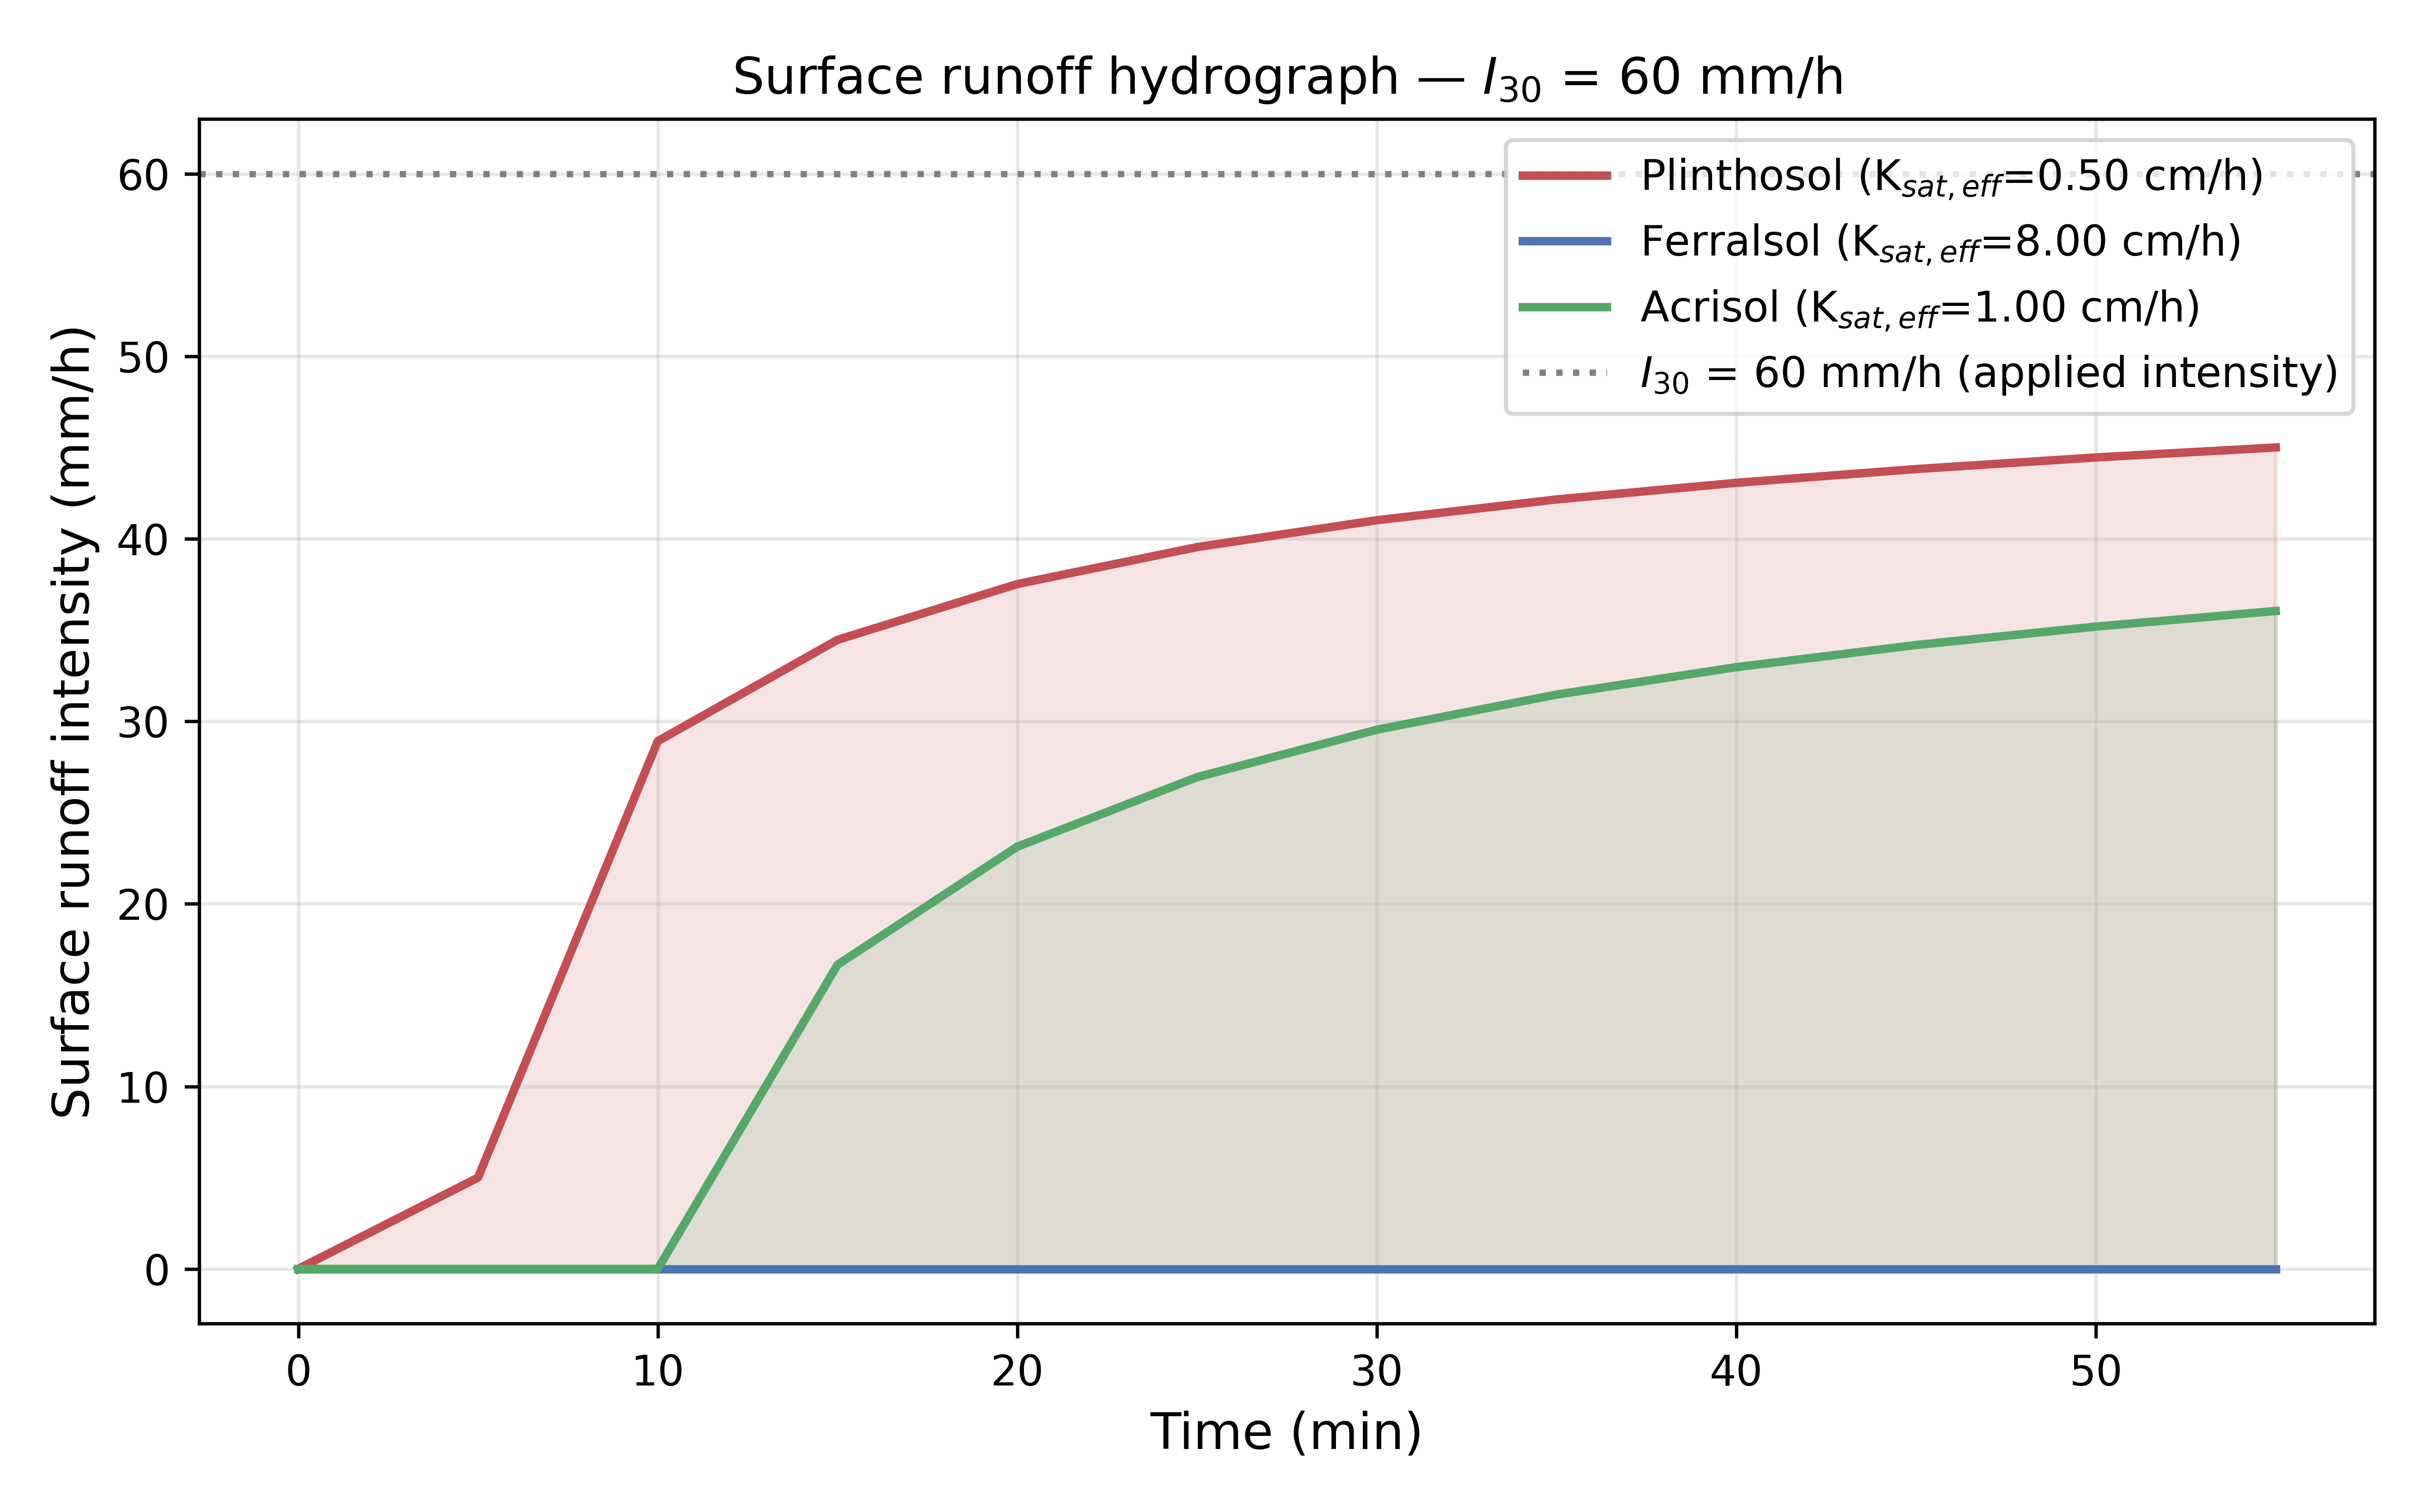
\includegraphics[width=0.8\textwidth]{figuras/fig_07_hidrograma_i60.png}
\caption{Hidrograma de escoamento superficial sob $I_{30} = 60$~mm/h para os três perfis de solo.}
\label{fig:hidrograma}
\end{figure}

\subsection{Erosão virtual e discrepância de $\delta$ (Teste~5)}

A discrepância média $\delta_{\mathrm{obs}}$ para o Plintossolo ($2{,}71 \pm 0{,}91$ para $I_{30} \geq 40$~mm/h) ficou abaixo do $\delta_{\mathrm{mod}} = 8{,}01$ predito com os parâmetros-alvo, gerando erro relativo de 66\% (Fig.~\ref{fig:erosao}c--d) e dimensionando a magnitude de calibração ainda necessária para que a RUSLE com $K_{\mathrm{plint}}$ se aproxime da resposta erosiva simulada por um modelo de desprendimento físico.

A superestimação é esperada porque os parâmetros ``verdadeiros'' ($n_1 = 1{,}0$, $\beta_{\max} = 2{,}5$ etc.) foram fixados em faixas plausíveis e não representam o sítio real. A mesma tendência se manifesta no Argissolo ($\delta_{\mathrm{obs}} = 0{,}61$ apenas para $I_{30} = 100$~mm/h, contra $\delta_{\mathrm{mod}} = 2{,}29$), enquanto a ausência de erosão no Latossolo ($\delta_{\mathrm{obs}}$ indeterminado por numerador zero) é consistente com $\delta \approx 1$ predito pelo modelo, reforçando a especificidade pedológica do fator de correção.

Uma segunda fonte de discrepância reside no modelo de desprendimento ($D = k_r(\tau - \tau_c)$), que não incorpora limitação por capacidade de transporte e pode subestimar $K_{\mathrm{obs}}$ em eventos extremos nos quais o sedimento é exportado da parcela antes de acumular. Em simulações com o WEPP, \citet{nearing_nicks_1998} identificaram comportamento análogo, com erosão predita excedendo a medida em eventos de alta intensidade quando a capacidade de transporte não era imposta como limitador. Em solos com fração de argila dispersível elevada, categoria que inclui Plintossolos pela presença de caulinita e baixa estabilidade estrutural subsuperficial, \citet{deviren_saygin_et_al_2018} demonstraram que a erodibilidade de desprendimento processual diverge da empírica da USLE.

\begin{figure}[htbp]
\centering
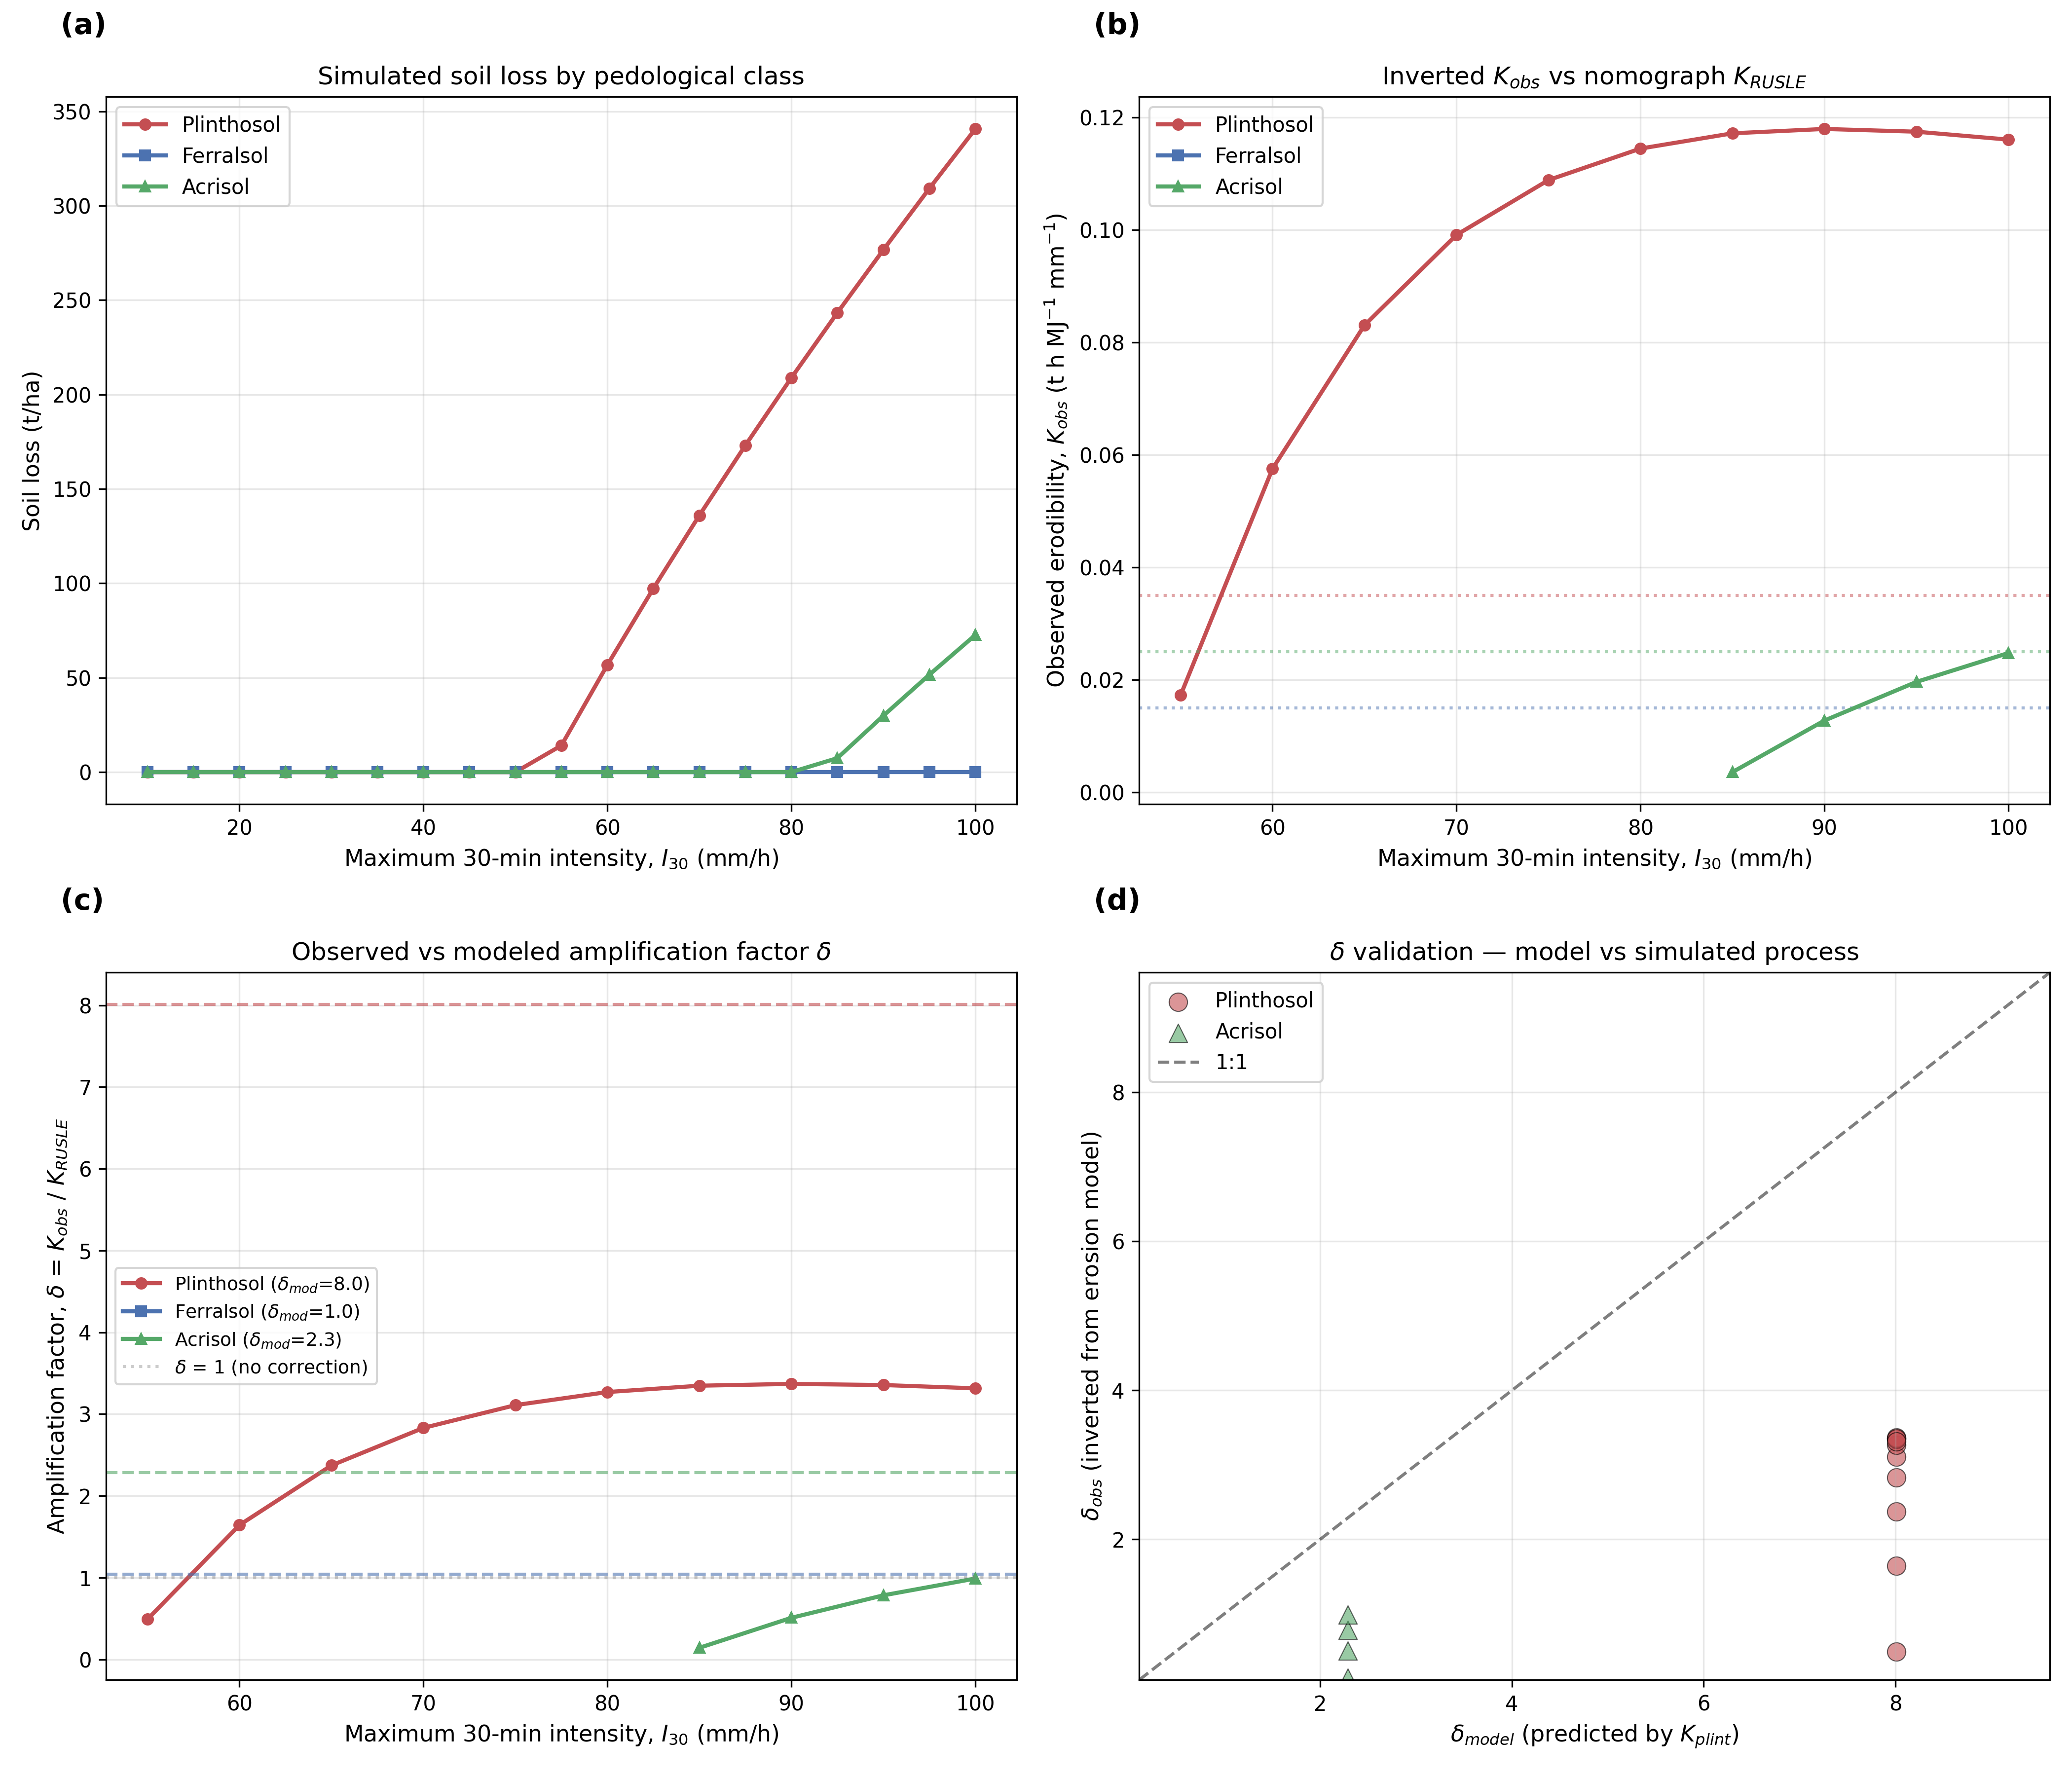
\includegraphics[width=\textwidth]{figuras/fig_08_erosao_virtual.png}
\caption{(a)~Perda de solo por classe pedológica e $I_{30}$. (b)~$K_{\mathrm{obs}}$ comparado com $K_{\mathrm{RUSLE}}$ (linhas pontilhadas). (c)~$\delta_{\mathrm{obs}} = K_{\mathrm{obs}}/K_{\mathrm{RUSLE}}$ versus $I_{30}$, com $\delta_{\mathrm{mod}}$ de referência (tracejadas). (d)~Validação $\delta_{\mathrm{obs}}$ versus $\delta_{\mathrm{mod}}$ (linha 1:1).}
\label{fig:erosao}
\end{figure}

A despeito da superestimação paramétrica, $K_{\mathrm{plint}}$ preserva a hierarquia pedológica (Plintossolo $>$ Argissolo $>$ Latossolo) e gera valores de $\delta$ estruturalmente consistentes com os processos simulados, resultado coerente com a premissa de que a estrutura multiplicativa captura a contribuição relativa de cada mecanismo amplificador mesmo quando os valores absolutos não estão calibrados \citep{renard_et_al_1997}. Os valores de $K_{\mathrm{obs}}$ de 0,058--0,116~t\,h\,MJ$^{-1}$\,mm$^{-1}$ obtidos para o Plintossolo situam-se no extremo superior da faixa documentada para solos brasileiros com horizonte subsuperficial limitante \citep{lafayette_cantalice_coutinho_2011,cassol_et_al_2023} e excedem em 2--8 vezes as estimativas originais do nomograma \citep{wischmeier_et_al_1971}.

A subestimação sistemática do nomograma da RUSLE em solos tropicais com processos subsuperficiais dominantes foi reportada por \citet{alewell_et_al_2019}, e \citet{torri_poesen_2014} já haviam apontado que a erodibilidade é propriedade emergente do perfil e não exclusivamente do horizonte superficial. Esse arcabouço sustenta a necessidade de fatores de correção que integrem informação pedológica em profundidade, tarefa que $K_{\mathrm{plint}}$ executa com cinco parâmetros e três variáveis de campo.

Em parcelas na Sicília, \citet{bagarello_et_al_2012} mediram 0,040--0,090~t\,h\,MJ$^{-1}$\,mm$^{-1}$ em solos com horizonte argiloso subsuperficial, faixa compatível com a obtida aqui apesar do contraste climático porque a descontinuidade textural gera impedimento hidráulico comparável em ambos os contextos. Em solos calcários com impedimento subsuperficial no Irã, \citet{ostovari_et_al_2016} relataram subestimação análoga, e no sul da Bahia \citet{francois_et_al_2024} identificaram $K$ como o parâmetro mais sensível da RUSLE. A convergência entre províncias geomorfológicas contrastantes sugere que $K_{\mathrm{plint}}$ pode ter aplicabilidade além dos Plintossolos, estendendo-se a solos cujo horizonte subsuperficial governa a resposta hidrológica.

A calibração de campo com dados de parcelas sob chuva natural pode ajustar os cinco parâmetros para minimizar a distância entre $\delta_{\mathrm{obs}}$ e $\delta_{\mathrm{mod}}$. O modelo de Green--Ampt assume frente de molhamento homogênea e $K_{\mathrm{sat}}$ efetivo único, e o déficit de umidade antecedente ($\theta_s - \theta_i$) e a curva de retenção introduzem incerteza adicional que pode afetar a magnitude absoluta do escoamento predito e, portanto, $\delta_{\mathrm{obs}}$. Um arcabouço bayesiano que incorpore priors geotécnicos de Rankine e a incerteza da curva de retenção pode mitigar tanto a equifinalidade residual de $k_3$/$n_3$ quanto a sensibilidade às premissas de Green--Ampt \citep{beven_freer_2001}.

\subsection{Envelope de ruído observacional e \emph{prior} de cobertura-manejo derivados de campanha exploratória de campo}
\label{sec:empirical-anchor}

A variabilidade observada no talude de Plintossolo desloca a calibração de $K_{\mathrm{plint}}$ para um regime mais heterogêneo que o representado pelo ruído sintético do Teste~1. As parcelas de solo descoberto e as parcelas com paliçadas baixas de pedra foram monitoradas em quinze coletas de sedimento entre 13 de maio e 24 de novembro de 2025. A precipitação acumulada extraída da série diária de 21~anos da estação climatológica do projeto (a menos de 500~m das rampas) atingiu 846,6~mm, equivalente a 77,5\% da média histórica anual de 1092~mm e correspondente a um $EI_{30}$ estimado de 2944,7~MJ\,mm\,ha$^{-1}$\,h$^{-1}$, cerca de 78\% da média regional de 3799~MJ\,mm\,ha$^{-1}$\,h$^{-1}$\,ano$^{-1}$. A produção média acumulada de sedimento foi de 2396,3~g por rampa de solo descoberto e 1024,4~g por rampa com paliçada baixa de pedra, equivalentes a 19,97 e 8,54~t\,ha$^{-1}$ respectivamente no intervalo monitorado. O coeficiente de variação entre as sete réplicas de solo descoberto médio foi de $\sim$80\%, valor compatível com a dispersão documentada por \citet{nearing_govers_norton_1999} em parcelas replicadas de erosão, nas quais pequenas diferenças de microtopografia, cobertura inicial e conectividade de fluxo ampliam a variância da perda de solo mesmo sob tratamento nominalmente idêntico.

Essa variabilidade não invalida a recuperabilidade demonstrada no Teste~1, mas indica que a calibração de campo tende a exigir modelos hierárquicos capazes de separar erro de medição, heterogeneidade entre rampas e resposta específica de cada evento. A razão solo descoberto/paliçada de 2,34 indica redução de sedimento mobilizado por uma barreira permeável fixa sob chuva e solo idênticos, mecanismo coerente com avaliações de cordões de pedra no norte da Etiópia, onde estruturas transversais reduziram a conectividade hidrossedimentológica por retenção a montante e encurtamento do comprimento efetivo de rampa \citep{nyssen_et_al_2007}. A resposta dessas barreiras, entretanto, varia com posição na encosta, redistribuição de sedimento e propriedades locais do solo, como observado por \citet{vancampenhout_et_al_2006}, de modo que a razão de 2,34 não representa eficiência universal de paliçadas, mas um \emph{prior} local de $C \cdot P \approx 0{,}43$ para estimar conjuntamente $K_{\mathrm{plint}} \cdot C \cdot P$ nas parcelas de Wischmeier instrumentadas. Como o modelo $K_{\mathrm{plint}}$ opera com $C = P = 1$ por definição, esse \emph{prior} evita atribuir à erodibilidade intrínseca uma redução de sedimento produzida por cobertura-manejo.

\begin{table}[htbp]
\centering
\caption{Restrições observacionais derivadas da campanha exploratória de campo e suas implicações para o desenho estatístico da fase de calibração do $K_{\mathrm{plint}}$.}
\label{tab:comparativa}
\small
\begin{tabular}{@{}l c c@{}}
\toprule
Restrição empírica & Valor observado & Implicação para o desenho da calibração \\
\midrule
CV entre réplicas de solo descoberto & $\sim$80\% & Modelos hierárquicos bayesianos preferíveis à regressão agrupada \\
Razão solo descoberto : paliçada de pedra & 2,34 & \emph{Prior} de $C \cdot P \approx 0{,}43$ para estimação conjunta de $K_{\mathrm{plint}} \cdot C \cdot P$ \\
Precipitação acumulada no intervalo & 846,6~mm (78\% do $EI_{30}$ anual) & Pluviógrafo de estação única suficiente para estimação do fator $R$ \\
Comprimento da rampa & 2,40~m & Comprimento integral de Wischmeier (22,13~m) requerido para $K_{\mathrm{obs}}$ não enviesado \\
Medição de escoamento & Ausente & Calhas Geib + tanques de armazenamento requeridos para particionar escoamento \\
Cálculo de $EI_{30}$ & Escalonado pela $P$ do intervalo & Registro por evento via cuba basculável requerido \\
\bottomrule
\end{tabular}
\end{table}


As limitações geométricas e instrumentais do arranjo exploratório, em especial o comprimento de rampa uma ordem de magnitude inferior ao padrão de Wischmeier, a ausência de medição de escoamento e o $EI_{30}$ escalonado pela chuva do intervalo em vez de calculado por evento isolado, restringem o uso direto desses dados para estimar $K_{\mathrm{obs}}$ não enviesado, mas não comprometem o papel da campanha como fonte de restrições observacionais para os cinco testes computacionais (Tabela~\ref{tab:comparativa}). O envelope de ruído de $\sim$80\% delimita a faixa em que a recuperabilidade paramétrica demonstrada no Teste~1 permanece útil para a calibração de campo, ao passo que a razão solo descoberto/paliçada de 2,34 quantifica empiricamente o fator cobertura-manejo associado a barreiras permeáveis fixas no mesmo regime hidrossedimentológico em que $K_{\mathrm{plint}}$ foi formulado. Em conjunto, os cinco testes computacionais e as restrições derivadas da campanha exploratória sustentam que a estrutura multiplicativa proposta é matematicamente identificável, fisicamente coerente com o gradiente pedológico tropical e empiricamente compatível com a variabilidade de campo observada em Plintossolos com erosão linear ativa, condições conjuntas que delimitam o escopo dos achados deste estudo e justificam a transição para a fase subsequente de calibração instrumental.
%% ================================================================
%%  5. CONCLUSÕES
%% ================================================================
\section{Conclusões}
\label{sec:conclusions}

Este estudo avaliou a identificabilidade paramétrica e a consistência física de uma correção multiplicativa de cinco parâmetros do fator $K$ da RUSLE ($K_{\mathrm{plint}}$) para Plintossolos com impedimento hidráulico subsuperficial, por meio de cinco testes computacionais ancorados em medições de campo de um Plintossolo Háplico e em perfis virtuais de Latossolo e Argissolo. A formulação proposta reproduziu a hierarquia de suscetibilidade entre as três classes pedológicas e preservou o nomograma de $K_{\mathrm{RUSLE}}$ como núcleo, amplificando-o apenas nas condições em que impedimento hidráulico, fitotoxicidade alumínica e vulnerabilidade geotécnica foram simultaneamente diagnosticados. Os parâmetros hidráulico-biológicos foram recuperáveis sob ruído observacional, ao passo que o par geotécnico apresentou equifinalidade restrita à faixa rasa de profundidade normalizada, mitigável por priors derivados da física de Rankine. O desenho multiclasse permitiu isolar a contribuição de cada amplificador, com o Latossolo operando como controle negativo, o Argissolo como controle parcial e o Plintossolo como caso de convergência dos três mecanismos. A análise de sensibilidade indicou domínio do termo hidráulico no Plintossolo e do termo fitotóxico no Latossolo, em coerência com o contraste pedológico entre as classes. Os resultados indicam que a correção multiplicativa é matematicamente identificável e fisicamente coerente nas condições simuladas, condição necessária para a etapa subsequente de calibração de campo. A transferência da formulação para Argissolos com gradiente textural abrupto, Plintossolos pétricos e Cambissolos rasos constitui extensão natural, pois essas classes compartilham descontinuidades pedológicas análogas e tendem a requerer apenas recalibração local dos cinco parâmetros.

%% ================================================================
%%  DECLARAÇÃO DE INTERESSES CONFLITANTES
%% ================================================================
\section*{Declaração de interesses conflitantes}

Os autores declaram não possuir interesses financeiros conhecidos ou relações pessoais que possam ter influenciado o trabalho relatado neste artigo.

%% ================================================================
%%  AGRADECIMENTOS
%% ================================================================
\section*{Agradecimentos}

Os autores agradecem à Universidade Federal de Sergipe e à Universidade Estadual de Feira de Santana pelo apoio logístico e à CAPES pela bolsa de pós-doutorado.

%% ================================================================
%%  DISPONIBILIDADE DE DADOS
%% ================================================================
\section*{Disponibilidade de dados}

Os scripts de simulação, parâmetros de entrada e figuras geradas estão disponíveis no Zenodo (\url{https://doi.org/10.5281/zenodo.19483403}). Os dados exploratórios de sedimento do talude e a série diária de 21~anos de precipitação estão disponíveis no repositório do projeto em \url{https://github.com/ldvsantos/palicada} (diretório \texttt{2-DADOS/}).

%% ================================================================
%%  FINANCIAMENTO
%% ================================================================
\section*{Financiamento}

Este trabalho foi financiado pela CAPES (bolsa de pós-doutorado).

%% ================================================================
%%  DECLARAÇÃO DE AUTORIA CRediT
%% ================================================================
\section*{Declaração de contribuição de autoria CRediT}

\textbf{Luiz Diego Vidal Santos:} Conceitualização, Supervisão, Administração do projeto, Redação -- revisão e edição. \textbf{Emersson Guedes da Silva:} Metodologia, Software, Análise formal, Curadoria de dados, Visualização, Redação -- rascunho original. \textbf{Marcos Oliveira Santos:} Investigação, Curadoria de dados. \textbf{Renisson Neponuceno de Araújo Filho:} Investigação, Recursos, Redação -- revisão e edição. \textbf{Henrique Antonio Silva:} Investigação, Validação. \textbf{Jémisson Mattos dos Santos:} Análise formal, Redação -- revisão e edição.

%% ================================================================
%%  MATERIAL SUPLEMENTAR
%% ================================================================
\section*{Apêndice A. Material suplementar}

O Material Suplementar~S1 contém a derivação completa da equação de altura crítica de Rankine utilizada na Seção~\ref{sec:test3}.

\bibliographystyle{elsarticle-harv}
\bibliography{../referencias_artigos}

\end{document}
